\chapter{Wearable Edge AI towards healthcare applications}
\label{chap:healthcare}

\nomenclature{CWS}{Cooperative Wearable System}
\nomenclature{FR-CWS}{Field Research Cooperative Wearable System}
\nomenclature{QoS}{Quality-of-Service}
\nomenclature{HUD}{Head-Up Display}

In this chapter, we evaluate the applications developed towards our second stakeholders. We defined them as researchers, physiologists, medical practitioners, patients and people which require health monitoring appliances. We also developed cyber-physical applications within three branches: physical condition monitoring, smart wearable systems in the context of COVID-19, and wearable-based human activity recognition.

\section{Physical condition monitoring in field}

The first approach in this context was applying the Wearable Edge AI context to monitor workers' conditions during field activities. This application relates to the healthcare monitoring section, but interfaces with the first interests. This happens as this study was developed as an integration from both stakeholder groups.

\subsection{Requirements}

The first step in this analysis is evaluating the requirements for the proposed method. For this matter, we display a version of the co-design diagram presented in Figure \ref{fig:simplified-codesign-4}, which is a simplification of the diagram presented in Figure \ref{fig:codesign-2.0}. 

\begin{figure}[ht!]
    \centering
    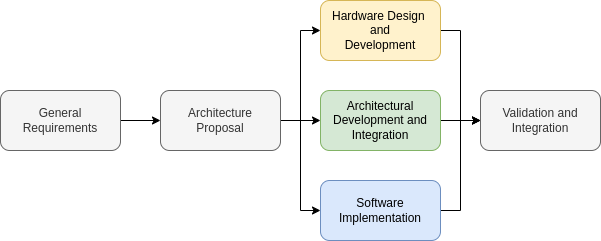
\includegraphics[width = .8\linewidth]{Figures/simplified-codesign.png}
    \caption{Simplified Co-design diagram.}
    \label{fig:simplified-codesign-4}
\end{figure}

This representation displays the need to raise the constraints for the application and classify them into the hardware, software or architectural domain. The constraints identified for this matter are:

\begin{itemize}
    \item This solution must gather data from the users and sense environmental conditions that can affect them [\textit{Hardware}].
    \item This solution must be integrated to personal protection equipment [\textit{Hardware}].
    \item The wearable devices must be able to communicate with mobile applications which will interpret their data [\textit{Architecture}].
    \item The communication needs to be efficient to stream the data through this local network [\textit{Architecture}].
    \item Data obtained from the applications must be processed in real-time [\textit{Software}].
\end{itemize}

In this case, we proposed a cooperative wearable system in which several users wear the proposed solution, which by itself serves for multiple purposes. In this case, often the answer for a constraint comes from the evaluation and development of others.

\subsection{Context Overview}

\begin{figure}[h!]
    \centering
    \includegraphics[width = .7\linewidth]{Figures/SAM_4593.JPG}
    \caption{Wearable Device Prototype, proposed in \cite{jp2019software}.}
    \label{fig:prototype}
\end{figure}

The system is built upon a prototype suggested by Amorim et al. \cite{jp2019software}, as illustrated in Figure \ref{fig:prototype}. We have not suggested any modifications to the hardware configuration as our goal is not to verify the device in isolation, but rather to assess the implementation of several devices. The sensors were previously employed in close proximity and evaluated during the prototype development phase.

We investigate the earlier proposal and validation of this solution. The development of innovative technologies necessitates a methodical procedure. In this context, we adhere to the notion of Multiple-User Cooperative Wearable Systems, which involves investigating the utilization of a single device across many applications.

Therefore, we utilize the understanding provided by the current sensors to outline innovative applications that can leverage this data to produce fresh insights. This study examines the progression of this system towards a Continuous Writing System (CWS), and more particularly, a French-English CWS (FR-CWS). This procedure adheres to the established protocols for the development and verification of wearable devices and systems. Moreover, we provide a hypothesis in which this system is capable of serving many devices.

This subsection provides the background in which we implement the suggested remedy. Initially, our wearable device gathers pertinent data from both the person and the immediate surroundings. Initially, this wearable device was specifically developed to provide assistance to workers in the open-sky mining sector \cite{jp2019software}. Therefore, this study examines a more extensive hypothetical situation in the field of forest studies. The creation process was informed by typical functions seen in wearable gadgets and field research. Under such circumstances, a team with expertise in multiple disciplines collects diverse information from the gadget. The individuals comprising this team are:


\begin{enumerate}
    \item A medic, monitoring the team's health \cite{sodhro2018energy, firouzi2018internet};
    \item A biologist/ecologist, measuring sensor values for his research \cite{costa2018abiotic, arena2018multiple, calvao2018land};
    \item A physiologist, studying the physical effort in each kind of task \cite{pereira2018physical, jahanbanifar2018evaluation, weeks2018implementing};
    \item A navigator, cross-checking the global position with physical or virtual maps \cite{velazquez2018outdoor, tjhai2018using, kiss2018navigation}.
\end{enumerate}\vspace{-6pt}

Every member of this group wears identical safety field research equipment and has access to the collective data of the entire team's gear. Furthermore, every member is provided with a Smartphone application that is tailored to their specific professional responsibilities, along with specially-designed features. This architecture aims to utilize the adaptable nature of the data generated by the device to cater to many topics using the same wearable, as a distinguishing feature of a multi-user Context-Aware System (CWS). 

\subsection{Wearable computing requirements}

This subsection provides a concise summary of the prerequisites for the specific circumstances in which this wearable system operates. The initial set of criteria is derived from the prevalent characteristics of wearable devices:

\begin{itemize}
    \item The device must not block the user's common movements;
    \item It must provide information from sensors;
    \item It must detect context changes.
\end{itemize}

Moreover, the integration of new equipment in field research necessitates the development of innovative AHPs. Therefore, it is preferable to integrate the wearable system with widely-used protective equipment. Utilizing these gadgets hinders the need for implanting a new safety device. Therefore, we selected a safety vest as the reference point for our suggested approach, using it as a case study.

From now on, the team will be designated as M for the medic, E for the ecologist, P for the physiologist, and N for the navigator. In order to meet the requirements of the interdisciplinary team, this gadget must be equipped with sensors that offer:

\begin{itemize}
    \item Body temperature and humidity (M, P);
    \item Heart rate and blood oxygenation (M, P);
    \item Environmental luminosity, temperature and humidity (M, P, E);
    \item Global Position and Altitude (E, N);
    \item Muscular Effort (P);
    \item Body Motion (M, P);
    \item Safety lights (M, E, N, P).
\end{itemize}

Each professional can obtain the required information from all the crew members, in an application designed with the specifications from each of them. This feature comes with the flexibility of CWS.

\subsection{Device Architecture \textcolor{black}{Description}}

In the preceding section, we outlined the prerequisites for the suggested CWS. Within this section, we will outline the structure and characteristics of the prototype utilized in this particular scenario. The diagram in Figure \ref{fig:devicearch} illustrates the primary components of this prototype.

\begin{figure}[h!]
    \centering
    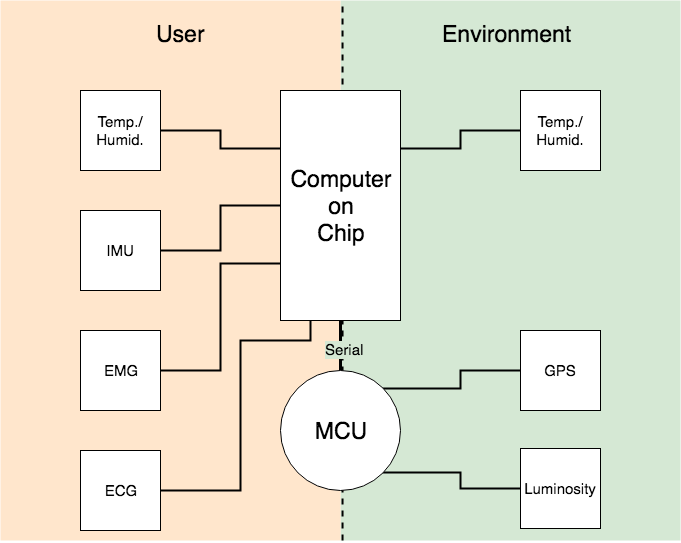
\includegraphics[width = .6\linewidth]{Figures/devicearch.png}
    \caption{Proposed device architecture.}
    \label{fig:devicearch}
\end{figure}

As mentioned, this device was previously presented by Amorim et al. \cite{jp2019software}. It has sensors to monitor both the user and some environmental variables. These sensors are:

\begin{itemize}
    \item User Sensors:\vspace{-6pt}
    \begin{itemize}
        \item \textbf{Temperature/Humidity Sensor}---This sensor monitors the temperature and humidity internally. This sensor connects reading digital data from a GPIO pin;
        \item \textbf{IMU Sensor}---This sensor monitors the user's body motion. It communicates using the I2C bus;
        \item \textbf{EMG Sensor}---This sensor monitors the muscular effort from the user. It transmits the measured data using GPIO monitoring;
        \item \textbf{ECG Sensor}---This sensor monitors the heart rate and blood oxygenation. It communicates using the I2C bus.
    \end{itemize}\vspace{-6pt}
    \item Environmental Sensors:\vspace{-6pt}
    \begin{itemize}
        \item \textbf{Temperature/Humidity Sensor}---This sensor monitors the temperature and humidity externally. This sensor connects reading digital data from a GPIO pin;
        \item \textbf{GPS Sensor}---This sensor gathers the global position data and transmits it to the computer board through the MCU. The MCU uses a serial connection to communicate with this board;
        \item \textbf{Luminosity Sensor} - This sensor gathers luminosity data and transmits it to the computer board through the MCU. The MCU uses I2C connection to communicate with this sensor.
    \end{itemize}
\end{itemize}\vspace{-6pt}

In addition, the vest offers the possibility of activation. The MCU can utilize the brightness sensor to trigger the activation of safety lights in the event that it detects a dimly lit environment. To enhance comprehension of the arrangement of sensors in this device, Figure \ref{fig:vest_illustration} depicts the spatial positioning of its components. As mentioned in the introduction of this section, this device underwent prior testing and validation in \cite{jp2019software}. The safety vest accommodates all the elements without obstructing or causing discomfort to the user.

\begin{figure}[h!]
    \centering
    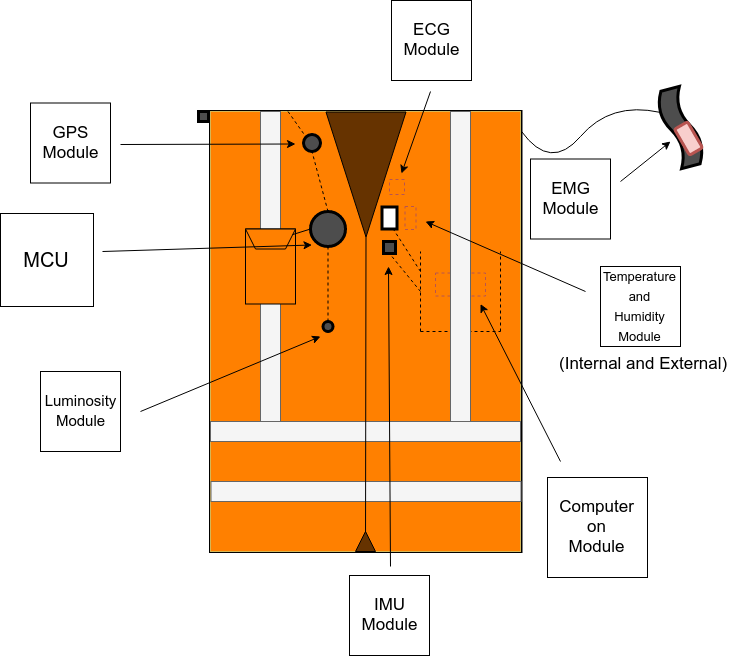
\includegraphics[width = .6\linewidth]{Figures/vest.png}
    \caption{\textcolor{black}{Wearable device illustration}.}
    \label{fig:vest_illustration}
\end{figure}

To have a more comprehensive understanding of the system's capabilities, it is crucial to chart the data acquisition time for each sensor. This information is also utilized to generate the simulated devices during the validation phase. In relation to this issue, we have condensed the duration of the procurement process for each sensor that is included in the prototype created by Amorim et al. \cite{jp2019software}. The summary is presented in Table \ref{tab:sapmlingtime}. Furthermore, we anticipate that the consuming applications will engage in additional post-processing of the data obtained from the sensors. Thus, the provided sampling times take into account the shortest interval necessary to obtain this essential information.

\begin{table}[h!]
\caption{\label{tab:sapmlingtime} Sampling time ratio for each sensor.}
\resizebox{\linewidth}{!}{%
\begin{tabular}{llll}
\toprule
 & Variable & Sensor & Sampling time \\ \hline
\multirow{4}{*}{User} & Temperature and Humidity & AM2302 (DHT22) \cite{dht22}& 2 s \\ \cline{2-4} 
 & IMU & MPU6050 \cite{mpu6050} & 0.125 ms \\ \cline{2-4} 
 & EMG & Myoware & System Sampling Rate \cite{raspizerow} ($\sim$5 $\mu$s) \\ \cline{2-4} 
 & ECG & MAX30100 \cite{max30100} & 1 ms \\ \hline
\multirow{3}{*}{Environmental} & Temperature and Humidity & AM2302 (DHT22) \cite{dht22} & 2s \\ \cline{2-4} 
 & GPS & FGPMMOPA6H \cite{fgpmmopa6h} & 0.1 s \\ \cline{2-4} 
 & Luminosity & TSL2561 \cite{tsl2561} & 2.5 $\mu$s \\ \hline
 \toprule
\end{tabular}%
}
\end{table}

This analysis used the provided information from the sensors and the computer-on-chip datasheets \cite{dht22, mpu6050, max30100, fgpmmopa6h, tsl2561, raspizerow}. \textcolor{black}{Finally, we consider that all sensors were properly calibrated in a previous assembly stage with the correct methods. For a broader comprehension, we also present the general characteristic of the calibration process for each sensor. The AM2302 sensor needs a chemical process in a closed chamber for calibration, as it is an hygrometer--thermometer \cite{waters2015updated}. The MPU-6050 is a 6-DoF IMU, which requires a 3-axis motion and spinning movements \cite{yadav2016fast}. As an EMG sensor, Myoware must be calibrated before the usage, considering reference levels of contraction signals \cite{oberg1995muscle}. As a GPS module, FGPMMOPA6H requires a factory calibration according to its antenna \cite{menge1998results}. TSL2561 is a lux meter, and therefore must also be previously calibrated with its response curve \cite{schrama1999novel}. Finally, MAX30100 is a pulse-oximeter, and thus requires factory calibration with the light wavelength response \cite{hayes2001new}.}

\subsection{System Architecture}

In the previous subsection, we outlined the key characteristics of the wearable devices that would form part of this system. Here, we introduce the suggested architecture for CWS. The architecture was derived from the collaboration of a multidisciplinary team. The crew consists of a medic (M), an ecologist (E), a physiologist (P), and a navigator (N), as previously stated.

This system adheres to the principle of Multiple-User Collaborative Writing System (CWS). In this particular setting, numerous individuals utilize a shared gadget. The increase in flexibility occurs at the application level, where the data obtained from the wearable devices will undergo post-processing. 

Figure \ref{fig:FR-CWS} depicts the integration of the CWS architecture. Each crew member possesses an application that collects data from the sensors over wireless communication protocols, as previously stated. The applications extract pertinent information for each individual involved in the process from the comprehensive dataset.

Wearable devices in contemporary applications can be regarded as Internet of Things (IoT) nodes, as evidenced by several studies \cite{wu2018we, varatharajan2018wearable, roopaei2018wearable, li2019wearable, nousias2018uncertainty, gia2018energy}. Therefore, within the framework of this study, each wearable device is also represented as an Internet of Things (IoT) node that forms a Fog-Radio Cloud Wireless System (FR-CWS) architecture. Every crew member has the ability to utilize a smartphone that is connected to the network or a gateway in order to access and get data from each wearable device.

Every crew member application requires a specific sampling interval based on their professional specialty. However, the sampling rate must take into account both the interval at which the sensor readings are taken and the inherent delay in communication, which is common in this type of system. Prior to proceeding, it is crucial to comprehend the communication alternatives for constructing a wireless network. Mahmoud and Mohamad~\cite{mahmoud2016study} categorize the network protocols for the Internet of Things (IoT) based on the communication range. They use the following terminology:


\begin{itemize}
    \item Proximity (up to 10 m);
    \item Wireless Personal Area Network (WPAN) (up to 100 m);
    \item Wireless Local Area Network (WLAN) (Up to 1,000 m);
    \item Wireless Neighborhood Area Network (WNAN) (up to 10 km);
    \item Wireless Wide Area Network (WWAN) (up to 100 km).
\end{itemize}\vspace{-6pt}

\begin{figure}[h!]
    \centering
    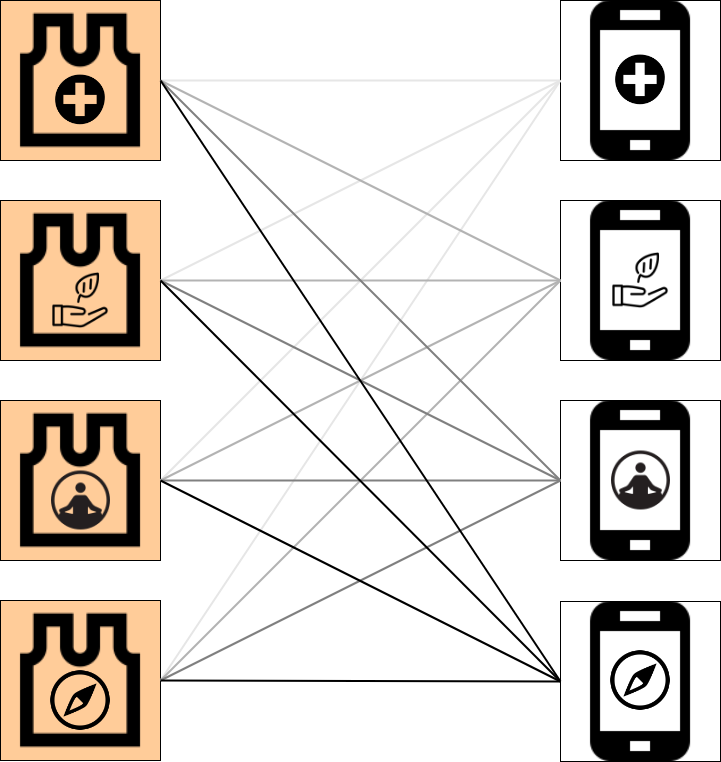
\includegraphics[width = .5\linewidth]{Figures/CFRWS.png}
    \caption{Field research cooperative wearable system architecture.}
    \label{fig:FR-CWS}
\end{figure}

According to the conjectured scenario, we desire that the users have access to each other data in distances within the ranges of WLAN and WPAN. For this matter, this work also provides some examples of technologies in use in these scenarios. Table \ref{tab:networks} presents these options.

\begin{table}[h!]
\centering
\caption{WPAN and WLAN connectivity technologies.}
\label{tab:networks}
\resizebox{\linewidth}{!}{%
\begin{tabular}{c|l|l|}
\cline{2-3}
\multicolumn{1}{l|}{} & \multicolumn{1}{c|}{Range} & \multicolumn{1}{c|}{Technologies} \\ \hline
\multicolumn{1}{|c|}{WPAN} & up to 100 m & \begin{tabular}[c]{@{}l@{}}bluetooth LE, ZigBee, Thread (6LoWPAM), Z-Wave, ANT$^+$,\\ WirelessHART, ISA100.11a (6LoWPAM), EnOcean, ...\end{tabular} \\ \hline
\multicolumn{1}{|c|}{WLAN} & up to 1,000 m & 802.11a/b/n/ac, 802.11af, 802.11ah \& 802.11p \\ \hline%please confirm if these is unit, if yes, please add blank spce between Numbers and units.
% these are not units, but indicators to network protocols, and formatted without blank spaces (https://ieeexplore.ieee.org/browse/standards/get-program/page/series?id=68)
\end{tabular}%
}
\end{table}

In a test scenario, we use the WLAN as connection mean, as it is enough to manage the information exchange for a crew working in proximity.


\subsection{Evaluation Methods}

Given that the proposed system operates as a dispersed device network, a crucial element of its architecture pertains to its communication limitations. In order to verify the effectiveness of this approach as a collaborative multi-node system, it is necessary to assess the practicality of the suggested system. Furthermore, it is vital to comprehend the constraints associated with the data accessibility within this network prior to formulating any algorithmic suggestion. Therefore, in this assessment, we establish a mathematical framework grounded in Quality-of-Service (QoS), akin to the models proposed by Boukerche and Samarah \cite{boukerche2008novel} and Silva and Oliveira \cite{silva2019analyzing}. This Quality of Service (QoS) test assesses the availability of information, taking into account the time restrictions that need to be considered when developing consuming applications.

At first, we assume that the transmission time is divided in equally-sized timeslots, represented by the set $T = \{t_1, t_2, t_3, ..., t_m\}$, where $t_{i+1} - t_i = \lambda$ for $1 < i \leq m$.

\begin{definition}
    Let $D = \{d_1, d_2, d_3, ..., d_n\}$ be the set of $n$ wearable devices present in the network.
\end{definition}

\begin{definition}
    Let $p_j = d_r...d_s$ be a data acquisition pattern, where each $d_i$ element is a device from $D$ ($d_i \in D$). 
\end{definition}

\begin{definition}
    Let $P = \{p_1, p_2, p_3, ..., p_k\}$ be a set of $k$ desired observation patterns.
\end{definition}

\begin{definition}
    Let $F(p_a, x)$ be the number of observations of a $p_a$ pattern within an $x$ number of timeslots.
\end{definition}

\begin{definition}
    Let $F(p_a)$ be the total number of observations of a $p_a$ pattern in the whole test period.
\end{definition}

The quality parameter $Q_s(p_i, k)$ for a pattern $p_i \in P$ expected in a $k$ number of timeslots is defined by the following equation:

\begin{equation}
\label{eq:qos}
    Q_s(p_i, k) = \frac{F(p_i, k)}{F(p_i)}.
\end{equation}

Each wearable device in our scenario will be emulated by utilizing a Raspberry Pi Zero W single-board computer connected to the network. The selection of these devices was based on their role as primary hardware nodes in the original prototype created by Amorim et al. \cite{jp2019software}.

Professionals may desire to receive communications from individual members, pairs of members, trios of members, or the entire crew in any given situation. If we define our pattern set $P$ as the set of all permutations of arrangements from the elements of $D$ according to this rule, then the size of our full pattern set is denoted by $S$:


\begin{align*}
    & S = P(4,1) + P(4,2) + P(4,3) + P(4,4),\\
    & S = \frac{4!}{3!} + \frac{4!}{2!} + \frac{4!}{1!} + \frac{4!}{0!},\\
    & S = 64.
\end{align*}

Consequently, we conducted 30 simultaneous tests for each device, aiming to acquire identical results, for every conceivable combination of $P$. During each test, the consumer applications simultaneously attempt to retrieve data from each sensor based on the potential message patterns of $P$. Every consumer application is created as a universal client within the network, capable of connecting to each node through the network gateway and retrieving its sensor data. Furthermore, during each test, the consumer applications will endeavor to collect identical data. Throughout the entire process, the wearable devices will be readily accessible, as they are a necessary component of both wearable technology and the Internet of Things.

Upon completion of the testing, we conduct a thorough analysis of the data to assess the quality elements as per the specified timing requirements. The string holding the simulated data will be released at regular intervals of 4.2 seconds for simulation purposes.


\subsection{Results}

In the previous part, we introduced the validation test set for the suggested case-study. Here, we examine the developed modules and practical features of the implemented tests. The test set being proposed is a simulated representation of the real network environment. To address this issue, we created a server application on four distinct computer-on-chip nodes, which are interconnected by a WLAN network. Furthermore, we set up four distinct computers as clients to retrieve data from the server nodes. 

The client nodes have the capability to execute a single query at any given time. This prevents a single application from causing the sensor nodes to become unresponsive after they are connected. As previously stated, every client application operates using identical code, and each sensor node carries out the same server function. The devices are disseminated throughout the local wireless network, as depicted in Figure \ref{fig:FR-CWS}.

We also said that the test encompasses every potential query case for each message. The evaluation approach takes into account the equation \ref{eq:qos}, which calculates the quality factor for a time frame consisting of $k$ timeslots. According to the information provided in Table \ref{tab:sapmlingtime}, it takes approximately 4.2 seconds to collect data from all sensors. Therefore, we opted to examine the discrete-time slots in intervals of $\lambda = 1$s. Furthermore, the quality factor must take into account the quantity of queries in a pattern, as each question will require a minimum of five timeslots to be resolved. Consequently, once the $k$ factor has been determined, the analysis employs the subsequent equation to compute the precise $k_l$ factor, where $n$ represents the quantity of queries in the $p_j$ pattern, $p_j \in P$:


\begin{equation*}
    k_l = n.k.
\end{equation*}

Furthermore, as previously stated, there exist a total of 64 distinct patterns when examining the individual combinations of each device $d_i$ from the set $D$. Hence, we gathered the durations for acquiring each pattern $p_j \in P$ that consists of a distinct arrangement of devices. 

Each of the four client devices performed this method 30 times, simultaneously and concurrently retrieving data from the server nodes. Ultimately, we examined the data by taking into account various values of $k$, commencing with $k = 5$. The results obtained from the tests are displayed in Figure \ref{fig:QoSresults}.

\begin{figure}[!h]
    \centering
    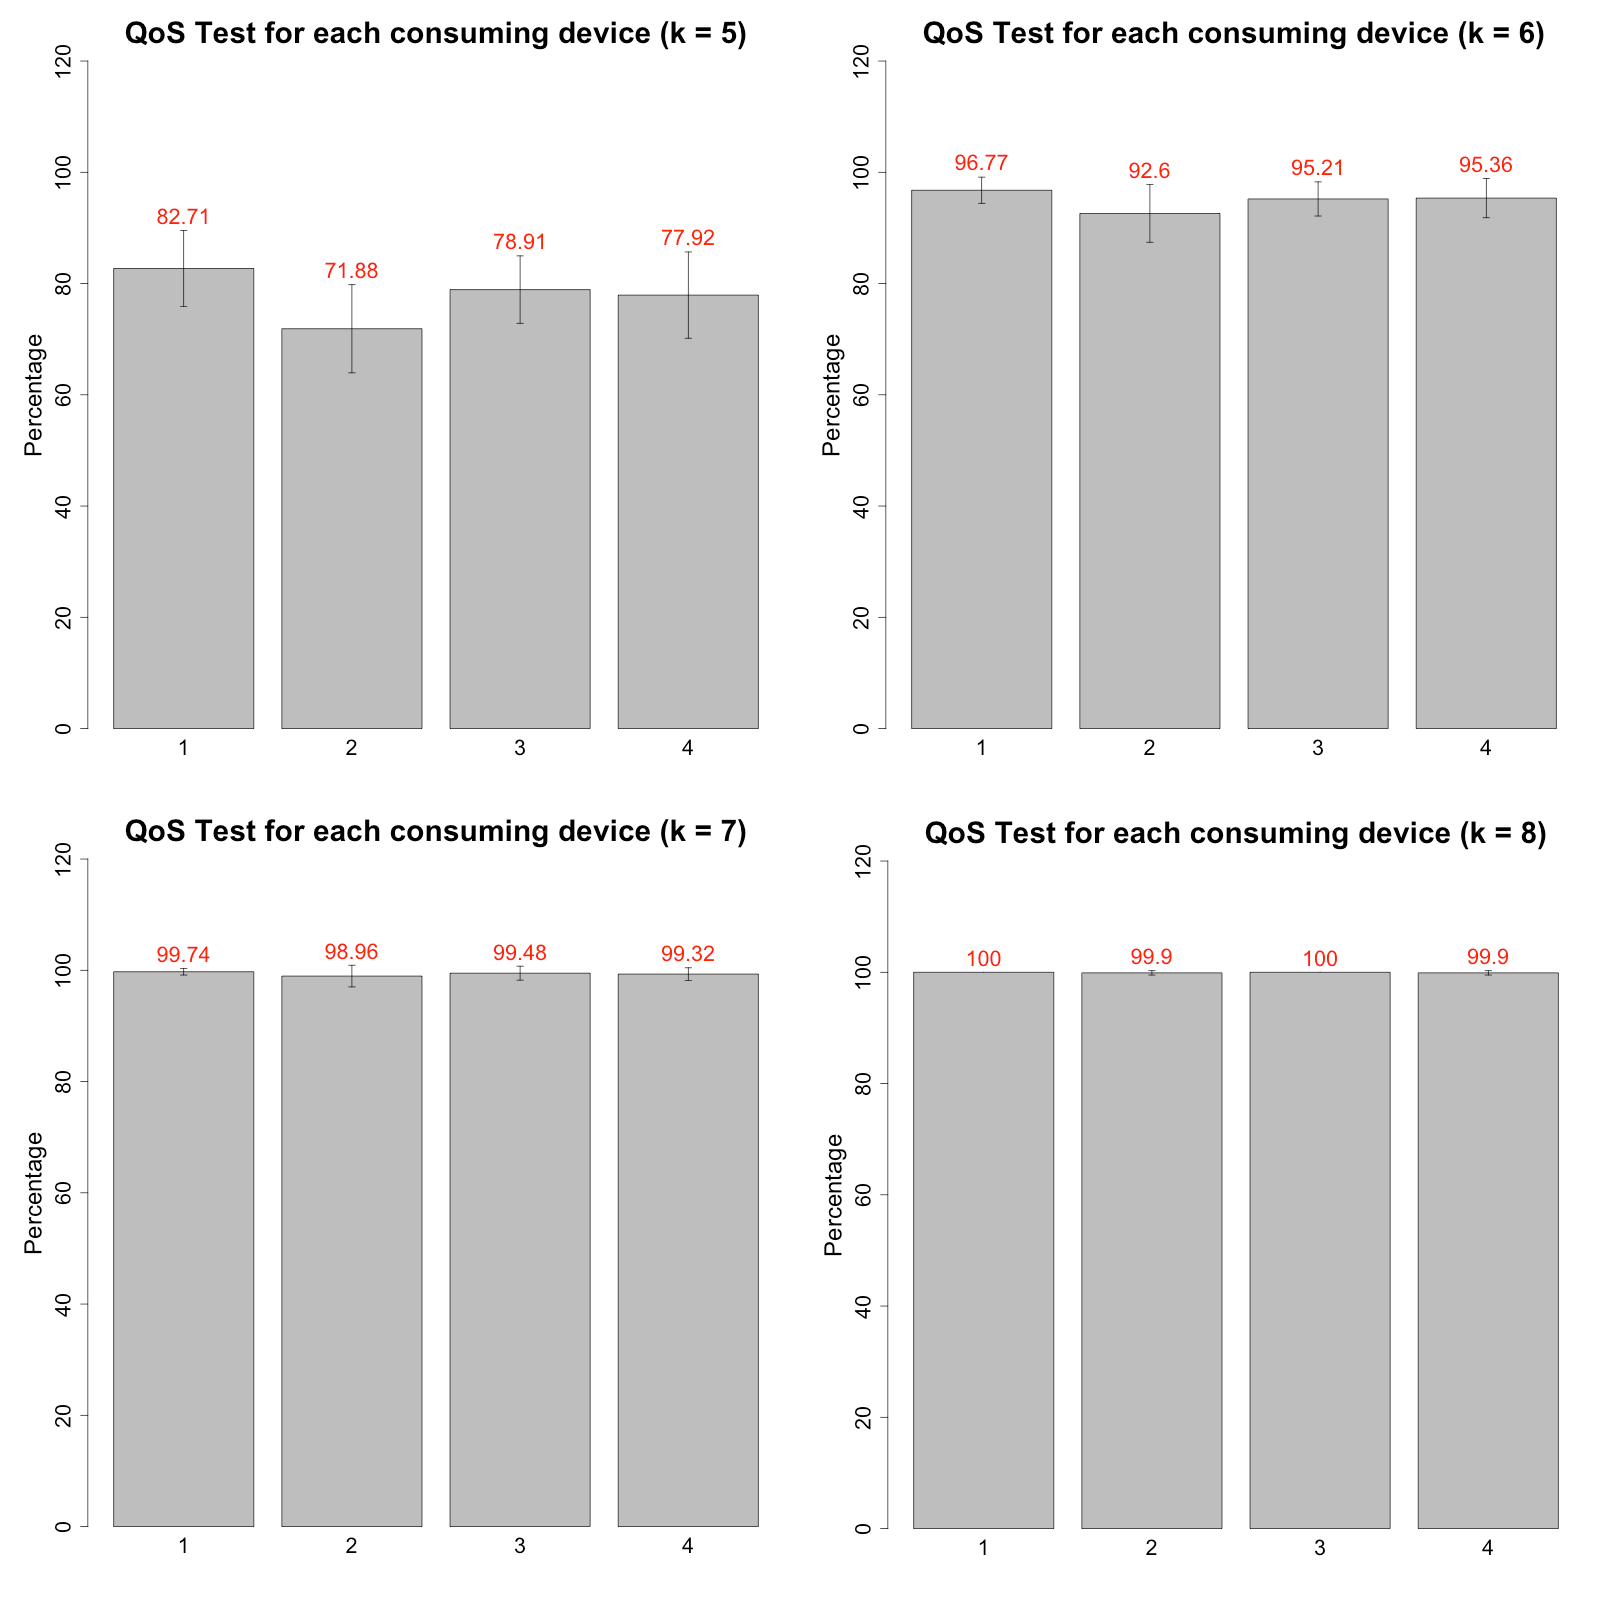
\includegraphics[width = \linewidth]{Figures/QoS_tests_result.png}
    \caption{Results of the QoS tests on each device.}
    \label{fig:QoSresults}
\end{figure}

The purpose of this study is to comprehend the limitations of the proposed architecture and its components. The QoS factor represents a proportion of the overall occurrences of a pattern. Consequently, we display the outcomes in the form of percentages.

The QoS tests reveal that a minimum of nine timeslots, equivalent to nine seconds, is required to ensure the full delivery of patterns. As previously stated, a minimum of five slots is required to generate and transfer the data. Therefore, it is essential for each study application to take into account the utilization of acquisition rates ranging from 5 to 9 seconds per device.

The results show that the average QoS factor for $k = 5$ is 77.8\%. The mean quality of service (QoS) factor for a given value of $k = 6$ is 95.0\%. The mean quality of service (QoS) factor for a given value of $k = 7$ is 99.4\%. The mean Quality of Service (QoS) factor for a value of $k = 8$ is 99.9\%. The quality factor is 100\% when the value of k is 9. As anticipated, decreasing the value of $k$ in the analysis leads to a deterioration in the quality factor outcome. This occurs as a result of the delay in sensor acquisition and the simultaneous use of the network. The graph labeled as Figure \ref{fig:QoS_average} illustrates the trend of the average factor for each value of $k$.

Another conclusion from this result is that the gain is small starting from $k = 7$. Increasing the number of timeslots from $k = 5$ to $k = 6$ elevates the average quality factor by 17.1\%. Increasing from $k = 6$ to $k = 7$ increases the quality factor in 4.4\%. Increasing from $k = 7$ to $k = 8$ raises the quality factor only by 0.5\%. Finally, increasing from $k = 8$ to $k = 9$ only elevates the quality factor by 0.1\%.

\begin{figure}[ht!]
    \centering
    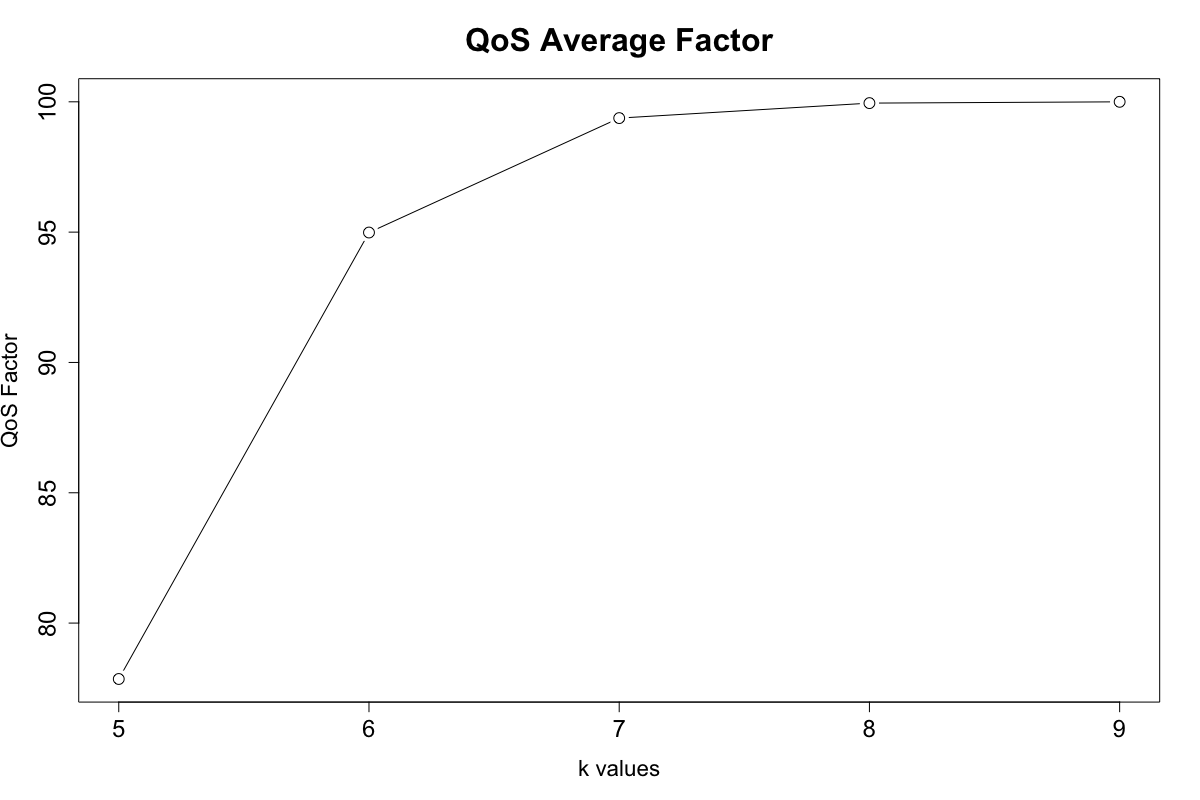
\includegraphics[width = .7\linewidth]{Figures/QoS-average.png}
    \caption{QoS average factor for each $k$ value.}
    \label{fig:QoS_average}
\end{figure}

The initial inference drawn from these test results confirms the validation of the network architecture. The test demonstrates the ability to simultaneously query wearable node devices for messages in an IoT-like application using wearable devices, even with the anticipated delay in sensor readings. This outcome validates the practicality of developing a Field Research Cooperative Wearable System within the specific case study. Moreover, when developing applications to utilize the data from the wearable nodes, it is important to take into account the timing limitations specified by the QoS test. Typically, the devices should aim to achieve an acquisition rate of approximately 7 seconds per node. Within the context of this text, employing a 7-second capture rate ensures a Quality of Service (QoS) factor of 99.4\%.

\section{Smart wearable systems in the context of COVID-19}

Due to advancements in hardware downsizing, the integration of Graphics Processing Units (GPUs), and the incorporation of Artificial Intelligence (AI) capabilities in System On Chip (SoC), wearable computers can now be categorized as edge computing devices as well (Chen, 2017). This viewpoint suggests improved and adaptable electronics and modular Computers-on-Chips. These devices have the capability to achieve greater involvement in local processing operations \cite{kim2017miniaturized}. In addition, due to their advanced networking capabilities, they are capable of transmitting data with a greater level of abstraction to applications that are based on edge servers or cloud platforms \cite{ren2017serving}. 

Context-awareness is a crucial element in wearable computing \cite{grubert2016towards}. Upon initial examination, this information pertains to the identification of alterations in the environmental circumstances within pervasive applications (Surve, 2017). Furthermore, an integral aspect of context-awareness is the monitoring of the user's conditions, sometimes referred to as user-awareness.

Kliger and Silberzweig \cite{kliger2020mitigating} state that COVID-19 is a viral illness caused by a newly discovered strain of coronavirus. The primary recognized symptoms include fever, cough, myalgia, and weariness. According to Prachand et al. (2020), a significant issue in combating the pandemic is the healthcare personnel' susceptibility to contamination hazards. However, Kliger and Silberzweig \cite{kliger2020mitigating} state that face masks and face shields are included in the list of recommended personal protection equipment (PPE) used by healthcare professionals to prevent contamination.

\subsection{Requirements}

The first step in this analysis is evaluating the requirements for the proposed method. For this matter, we display a version of the co-design diagram presented in Figure \ref{fig:simplified-codesign-5}, which is a simplification of the diagram presented in Figure \ref{fig:codesign-2.0}. 

\begin{figure}[ht!]
    \centering
    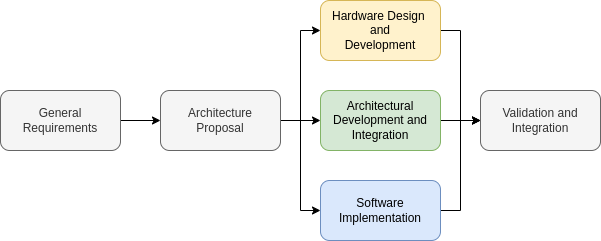
\includegraphics[width = .8\linewidth]{Figures/simplified-codesign.png}
    \caption{Simplified Co-design diagram.}
    \label{fig:simplified-codesign-5}
\end{figure}

This representation displays the need to raise the constraints for the application and classify them into the hardware, software or architectural domain. The constraints identified for this matter are:

\begin{itemize}
    \item This solution must gather data from the users and sense gather information using external markers [\textit{Hardware}].
    \item This solution must be integrated to personal protection equipment [\textit{Hardware}].
    \item The wearable devices must have low current consumption for an increased autonomy [\textit{Hardware}].
    \item The integration of data from multiple devices must happen within and edge server [\textit{Architecture}].
    \item The communication needs to be efficient to stream the data through this local network [\textit{Architecture}].
    \item Data obtained from the applications must be processed in real-time [\textit{Software}].
\end{itemize}

In this section of our work, we propose the architecture for a novel wearable appliance to help the professionals in the frontline of the COVID-19 engagement. The proposed appliance has two main goals. The first one is to gather information from environment signals using a camera as a smart sensor. The other one is to monitor the medical professionals' health conditions using internal measurement sensors. We also prototyped a version of the proposed architecture to test its feasibility and features.

\subsection{{Architecture Proposal}}

Here, we utilize this knowledge to suggest a new advanced structure for the wearable device. We choose the protective face shield as the foundation for this architecture development. This item is a safety face shield that has been modified to include a Head-Up Display (HUD). This viewpoint advocates for the implementation of an additional protective barrier, as advised by the World Health Organization (WHO), to safeguard against direct contamination \cite{world2020advice}. Moreover, the suggested appliance aims to offer context-awareness, taking into account both the environmental conditions and the user's awareness.

\begin{figure}[h!]
    \centering
    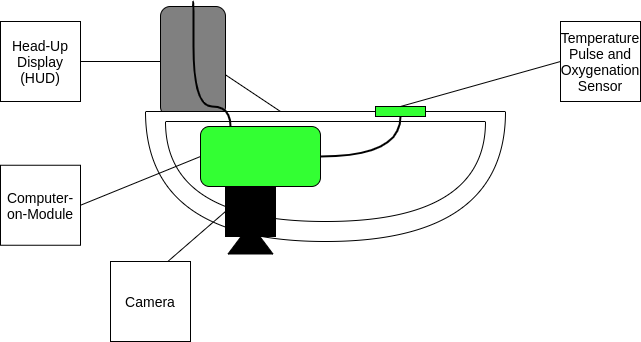
\includegraphics[width = .6\linewidth]{Figures/fs-schematics.png}
    \caption{Schematic View of the Proposed Prototype}
    \label{fig:fs-schematic}
\end{figure}

The suggested design consists of three main components: an environmental sensing element, a health monitoring sensor, and a heads-up display (HUD) interface. The integration of all these parts is achieved by the utilization of an integrated computer-on-module, which is powered by a battery. Figure \ref{fig:fs-schematic} depicts a schematic representation of the arrangement of elements. To perceive the surroundings, we suggest use a camera. Initially, this sensor enables remote access to the medical records of patients. 

The internal application utilizes a QR-Code to identify the patient and presents the most pertinent information via the Heads-Up Display (HUD). To detect the user's health status, we suggest utilizing a pulse-oximetry and temperature sensor. This module offers data regarding users' temperature, blood oxygenation, and pulse conditions over the course of usage. 

The user awareness interface is an integrated heads-up display (HUD). The device utilizes a compact Organic Light-Emitting Diode (OLED) screen with a partially reflective surface and a lens to create the intended transparent look. Due to the compact size of the display, it can only accommodate a restricted amount of information. These pieces integrate with an ARM-based single-core computer-on-module. This board possesses wireless networking capabilities for seamless integration with the local network. This functionality enables the transfer of the user's data and the retrieval of information regarding patients that are kept in the local servers. 

\subsection{{Prototyping and Validation Tests}}

This section presents the produced prototype to validate this idea and the tests used to evaluate its performance. 

\subsubsection{Prototype Description}

\begin{figure}[h!]
    \centering
    \includegraphics[width = .5\linewidth]{Figures/max30100.JPG}
    \caption{Pulse-Oxymeter and Temperature Sensor Placement}
    \label{fig:max30100}
\end{figure}

Initially, we commenced the production of the prototype by utilizing a 3D-printed face shield foundation. Volunteers utilize this basis to fabricate face shield masks. Upon this foundation, we established all the essential components required to develop the suggested application. The computer-on-module utilized was a Raspberry Pi Zero W. The solution is equipped with a solitary ARMv7 processing core, which is integrated within a Broadcom BCM2835 chipset. This CPU has a clock frequency of up to 1GHz. The device is equipped with 512MB of RAM and a wireless board that supports an 802.11 b/g/n WLAN connection, Bluetooth 4.1, and BLE protocols. We utilized a plastic enclosure to organize the computer-on-module and established connections to the remaining components via cables. The total weight of the solution, including the battery, is around 200g.

\begin{figure}[h!]
    \centering
    \includegraphics[width = .5\linewidth]{Figures/display.JPG}
    \caption{HUD See-through Display}
    \label{fig:display}
\end{figure}

We employed a MAX30100 pulse-oximeter to detect and monitor the patients' health status. This sensor supplies data necessary for computing the users' heart rate, blood oxygen saturation, and body temperature. The device is powered by a 3.3V output generated from the computer-on-module and communicates through an I$^2$C/SMBus serial link. The positioning of this sensor in the prototype is seen in Figure \ref{fig:max30100}. We employed a Raspicam V2 module\footnote{\url{https://www.raspberrypi.org/documentation/hardware/camera/}} to perceive the surroundings. This device features an 8-megapixel picture resolution, with video formats of 1080p, 720p, and 480p. It can be accessed using the V4L2 Linux driver. The device offers a horizontal field-of-view of 62.2 degrees and a vertical field-of-view of 48.8 degrees. This device establishes a connection with the central computer through the utilization of the MIPI camera serial interface.

The user interface is a Heads-Up Display (HUD) that presents information directly in front of the user's right eye. In this example, we utilized a 96x64 pixels OLED display\footnote{\url{https://img.filipeflop.com/files/download/Datasheet\_SSD1331.pdf}} enclosed within a 3D-printed casing. This module utilizes an SPI serial interface for communication. A semi-reflexive membrane was employed to form the reflexive surface, positioned in front of an acrylic layer. We positioned a lens with the accurately computed focal length to exhibit the information at the precise distance. Figure \ref{fig:display} illustrates the information that may be accessed using this particular model of the transparent display.

\begin{figure}[ht!]
    \centering
    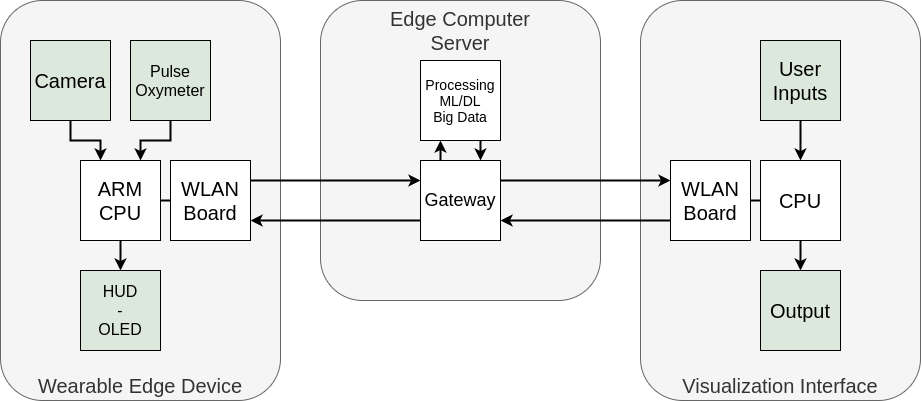
\includegraphics[width = .7\linewidth]{Figures/dataflow.png}
    \caption{Data Flow for the Proposed Prototype}
    \label{fig:dataflow}
\end{figure}

The computer-on-module consistently collects data from its sensors. Utilizing its wireless functionalities, it transmits this data to a server for storage and retrieves specific information based on the observed data. Ultimately, it generates the feedback frame of the HUD screen based on the received response and the data from the sensors. Figure \ref{fig:dataflow} illustrates the flow of data within the systems, based on the information depicted in this section.

\subsubsection{Validation Tests}

Here, we introduce the test set that was utilized to validate the proposed solution. In order to evaluate the system, we will conduct tests on several elements. A wearable appliance refers to a gadget that has limited energy resources available to it \cite{hong2019wearable,gia2018energy}. Furthermore, the utilization of processing power is a significant limitation in this particular situation \cite{soros2015fast}. Additionally, we aim to verify some functioning features of the system. Therefore, our test set takes into account:

\begin{enumerate}
    \item A \textbf{current consumption profiling test}, to observe how the proposed device behaves due to processing charge;
    \item A \textbf{full battery discharge test}, for probing the energy constraint and autonomy;
    \item A \textbf{functional validation test}, to observe how the system reads the provided data.
\end{enumerate}

In the initial two tests, we employed a data collecting device to deliver instantaneous data on consumption by utilizing a sensor and a microcontroller. The sensor utilized was an INA219 current consumption sensor, whereas the microcontroller employed was an Arduino Uno. The configuration for this probe is shown in Figure \ref{fig:probe-config}.

To obtain a singular output result, we calculate the mean measurement of 20 samples taken at an approximate rate of 100 samples per second. The ultimate sampling rate for acquiring a singular value was roughly 4.5 samples per second.

\begin{figure}[h!]
    \centering
    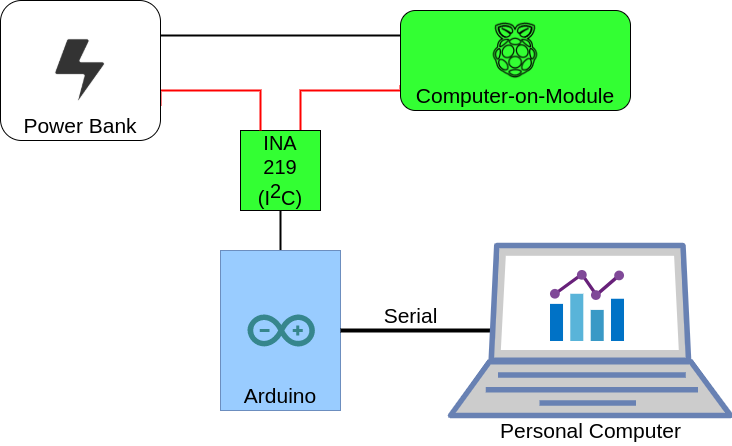
\includegraphics[width = .6\linewidth]{Figures/test-schematics.png}
    \caption{Current Consumption Probe Configuration}
    \label{fig:probe-config}
\end{figure}

In the \textbf{current consumption profiling test}, we observe how the system consumes energy in different stages of its functioning. For this matter, we performed a current consumption test considering various stages of the system functioning. We performed a 210-second run using a 5V power source. In this experiment, the device runs the following states in the approximate time intervals:

\begin{enumerate}
    \item Device off -- 0s-10s;
    \item Boot -- 10s-65s;
    \item SSH enabled -- Idle -- 65s-110s;
    \item Run application -- 110s-180s;
    \item SSH enabled -- Idle -- 180s-200s;
    \item Device off -- 200s-210s.
\end{enumerate}

Using this metric, we anticipate examining the present consumption of the many potential states of the system. Furthermore, we anticipate gaining a more comprehensive understanding of the system's energy limitations. In order to enhance understanding, we also conduct the subsequent test as described.

During the \textbf{full battery discharge test}, we anticipate examining two distinct facets. Initially, our objective is to assess the level of autonomy of the system based on a certain power source. Additionally, we aim to assess the consistency of consumption during the entire duration of execution. This assessment takes into account both quantitative and qualitative characteristics. The current consumption, without significant increases, primarily demonstrates the resilience of the behavior. Furthermore, it is imperative to ascertain the level of autonomy exhibited by this system, taking into account the various constraints that have been mentioned.

Additionally, we do a \textbf{functional validation test}. Through an analysis of the system's essential components, we assess its practicality and explore potential extra features. We evaluate sensing technologies that are capable of detecting both user-awareness and environment-awareness. Our analysis focuses on the extraction and transmission of information to an external edge server appliance. We facilitate the utilization of Edge AI to assess the characteristics of the provided data within this device.

\subsection{{Validation Tests Results}}

In this section, we present the results for these tests and preliminary discussions and conclusions.

\subsubsection{Current Consumption Profiling Test}

The first proposed experiment is the current consumption profiling test. In this scope, we want to describe the functioning of the system throughout different stages. For this matter, we divided the test time into six stages: Device off (1), Boot (2), SSH enabled - Idle (3), Run application (4), SSH enabled - Idle (5), and Device off (6). This test represents roughly a ``symmetrical'' startup, execution, and shutdown from the prototype. Figure \ref{fig:cptest} displays the results obtained from this experiment.

\begin{figure}[h!]
    \centering
    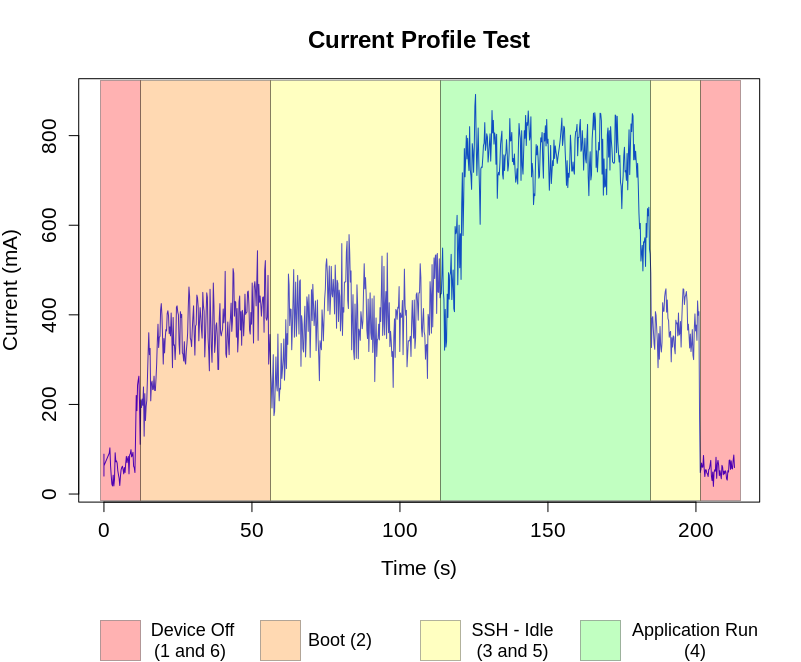
\includegraphics[width = .8\linewidth]{Figures/cptest-f.png}
    \caption{Current Consumption Profiling Test Result}
    \label{fig:cptest}
\end{figure}

In red, we display the probe readings when the system was off (Stages 1 and 6). These results display some noise but roughly represent the ``zero-state'' of this system. In orange, we display the current consumption results in the system boot (Stage 2). In this case, it is possible to see that the reading values increase until reaching a stable state.

In yellow, we display the results for the ``SSH enabled - Idle'' stages (3 and 5). In these intervals, the system was on, and the ssh connection was established. Nonetheless, the application was not running yet, configuring an idle state. At the connection establishment, we observe some instability in the current consumption, which reaches a stable state right after.

Finally, in green, we display the current consumption result for the application run time. In this case, the device starts the application, acquiring and transmitting data. In this case, the prototype is consuming the fully required resources. From the data, it is possible to see that the current increases during the system start-up, reaching a stable state after some seconds. The system also displays a slope decrease on the current, reaching a stable level in the shutdown's idle state. Table \ref{tab:cprofiling-test} displays the average current consumption for each stage.

\begin{table}[h!]
\centering
\caption{Profiling Test Results}
\label{tab:cprofiling-test}
\resizebox{0.6\linewidth}{!}{%
\begin{tabular}{llll}
\cline{2-4}
 & \multicolumn{3}{c}{\textbf{Current (mA)}} \\ \cline{2-4} 
 & min. & max. & avg. \\ \hline
Stage 1 & 3 & 86 & 45.53 $\pm$ 22.27 \\ \hline
Stage 2 & 56 & 529 & 331.4 $\pm$ 86.6 \\ \hline
Stage 3 & 232 & 565 & 384.4 $\pm$ 65.8 \\ \hline
Stage 4 & 744 & 927 & 831.4 $\pm$ 32.6 \\ \hline
Stage 5 & 268 & 444 & 359.5 $\pm$ 45.0 \\ \hline
Stage 6 & 3 & 73 & 40.63 $\pm$ 14.0 \\ \hline
\end{tabular}}%
\end{table}

\subsubsection{Full Battery Discharge Test}

Following the analysis of the current consumption for each stage, we proceeded to conduct a discharge test. For this experiment, we utilize a compact battery as a potential power source for the device and assess its duration and mean electrical usage. Figure \ref{fig:discharge} exhibits the measurement outcomes during the entire duration of the test.

\begin{figure}[!h]
    \centering
    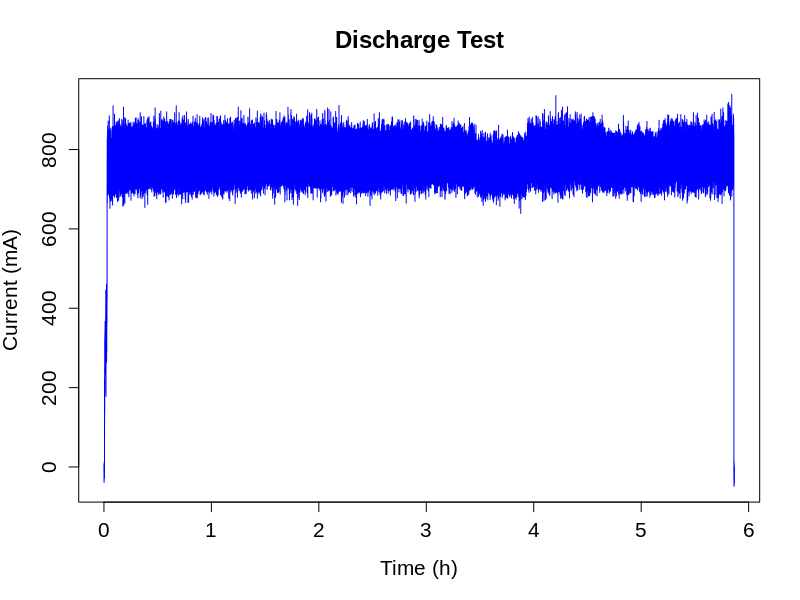
\includegraphics[width = .6\linewidth]{Figures/discharge.png}
    \caption{Discharge Test Result}
    \label{fig:discharge}
\end{figure}

For this test, we utilized a 4000 mAH power bank with a low weight as the primary battery for the system. The mean current during the test was 779.3 $ \pm $ 58.7 mA, with a recorded maximum of 939 mA. The prototype exhibited consistent performance throughout the whole test, indicating a high level of robustness for this device. Additionally, the autonomy was approximately 6 hours of continuous operation. These results support the findings of the profiling test, confirming the viability of the solution and its predictable behavior. This information also enables the choice of a suitable power source based on the current needs of healthcare personnel.

\subsubsection{Functional Validation Test}

Ultimately, we conducted a functional validation of the prototype to assess its viability in a situation that closely resembles the context of the end user. The intended appliance aims to retrieve two distinct types of information. Our objective is to utilize a camera to perceive data from the surroundings and employ a built-in sensor to retrieve information from the user.

Initially, we assessed the practicality of the external sensor. At first, it functions solely as a detector for a QR code to access information from other advanced sensors. Therefore, our hypothesis regards the wearable camera as a sensor that extracts images. The system obtains and transmits frames to an edge computing server for processing.

To address this issue, we incorporated a streamer program into the device. Therefore, the edge computing server has the capability to promptly establish a connection with the wearable device, get a single frame, and analyze it in order to locate a QR code containing an identifying query. Consequently, we created a straightforward program capable of extracting data from the wearable device and analyzing it for a QR code. The ultimate outcome for this example is depicted in Figure \ref{fig:qr-code-validation}.

\begin{figure}[!h]
    \centering
    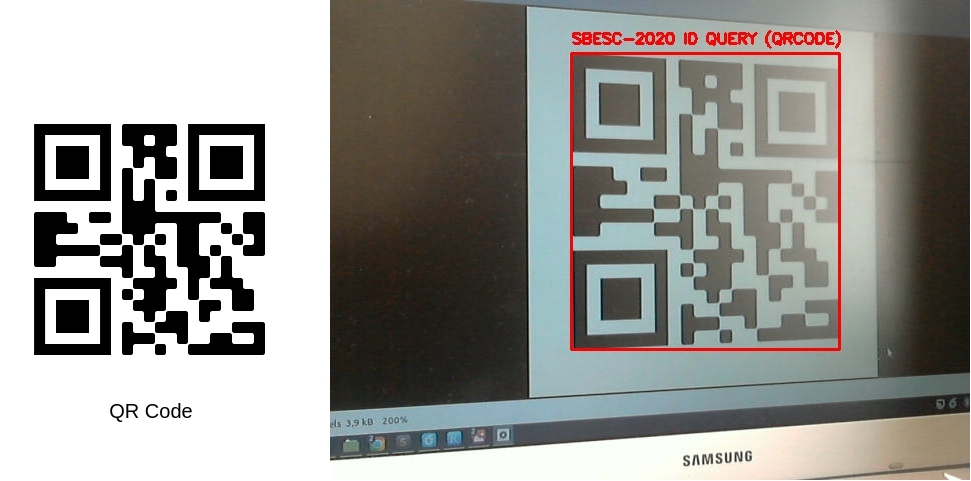
\includegraphics[width = .7\linewidth]{Figures/validation-1.png}
    \caption{QR Code Acquisition Validation}
    \label{fig:qr-code-validation}
\end{figure}

Following the validation of the external data collecting procedure, it was necessary to also validate the acquisition of the user's health conditions data. For our prototype, we utilized the MAX30100, a device that offers data on temperature and pulse-oximetry. This application utilizes a wearable device to compute the blood oxygen saturation (SpO$_2$) data by analyzing measurements obtained from infrared and red light emitting diode (LED) pulses. Hemoglobin exhibits differential absorption of red and infrared light depending on the presence or absence of oxygen. Figure \ref{fig:max30100-data} depicts the sampling readings of the probe sensor, which were taken at a rate of around 23 samples per second for a duration of approximately 15 seconds. The blue line represents the measurements of the infrared pulses, while the red line represents the measurements of the red light pulses.

\begin{figure}[h!]
    \centering
    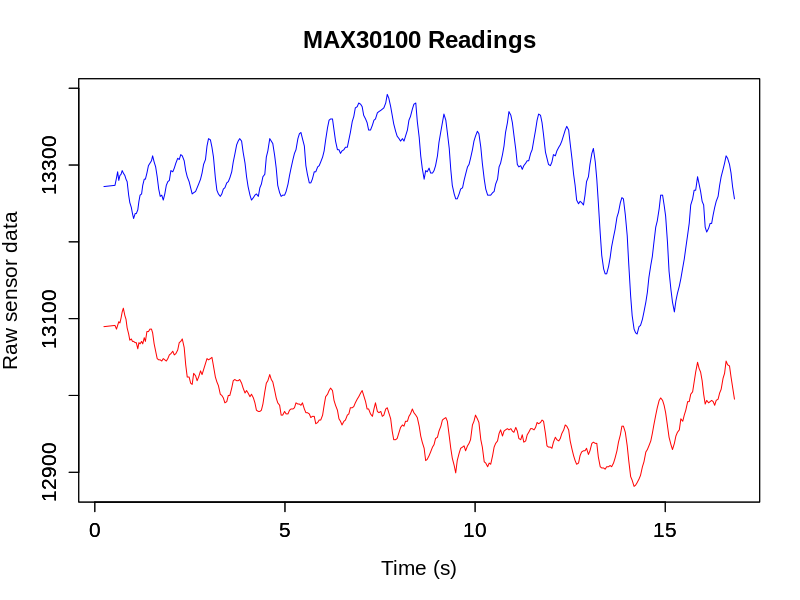
\includegraphics[width = .6\linewidth]{Figures/max30100-data.png}
    \caption{MAX30100 Probe Readings}
    \label{fig:max30100-data}
\end{figure}

\begin{figure}[h!]
    \centering
    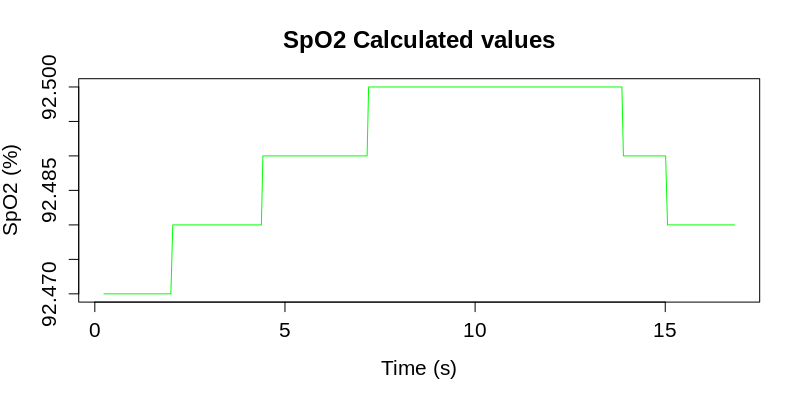
\includegraphics[width = .6\linewidth]{Figures/SPO2.png}
    \caption{SpO$_2$ Readings Obtained from the Computer-on-Module}
    \label{fig:spo2}
\end{figure}

Usually, the data can be analyzed by considering the AC components that have been adjusted for the DC components \cite{tremper1989pulse}. The computer-on-module processes the readings as SpO$_2$. Figure \ref{fig:spo2} displays the data obtained from the computer-on-module. The pulse information can be acquired by simply enumerating the number of crests within a designated time interval. The collected data can be subsequently assessed on the edge computing server appliance using machine learning techniques to examine the temporal sequences.

The analyses conducted on the prototype ensure the functional and non-functional validation of every part of the proposed architecture. We conducted a functional analysis to confirm that the prototype can be successfully integrated into the proposed appliance by verifying its key components. Non-functional analysis involves identifying the limitations that must be met for the proposed system to operate effectively.

\subsection{Edge Computing - Architecture Proposal}

Typically, edge devices are used in a wireless network environment to carry out cooperative duties, which is commonly linked to the Internet of Things (IoT) concept \cite{long2017edge}. Therefore, the initial determination in this suggestion for the system's architecture is the networking environment. Given the need for rapid adaptation and deployment of structures like mobile field hospitals \cite{chen2020mobile}, an optimal approach would be to utilize a portable solution for swiftly establishing a management framework. The solution's network type is a Wireless Local Area Network (WLAN), as determined by the required connectivity ranges \cite{mahmoud2016study}. The main planned design is depicted in Figure \ref{fig:gen-arch}.

\begin{figure}[h!]
    \centering
    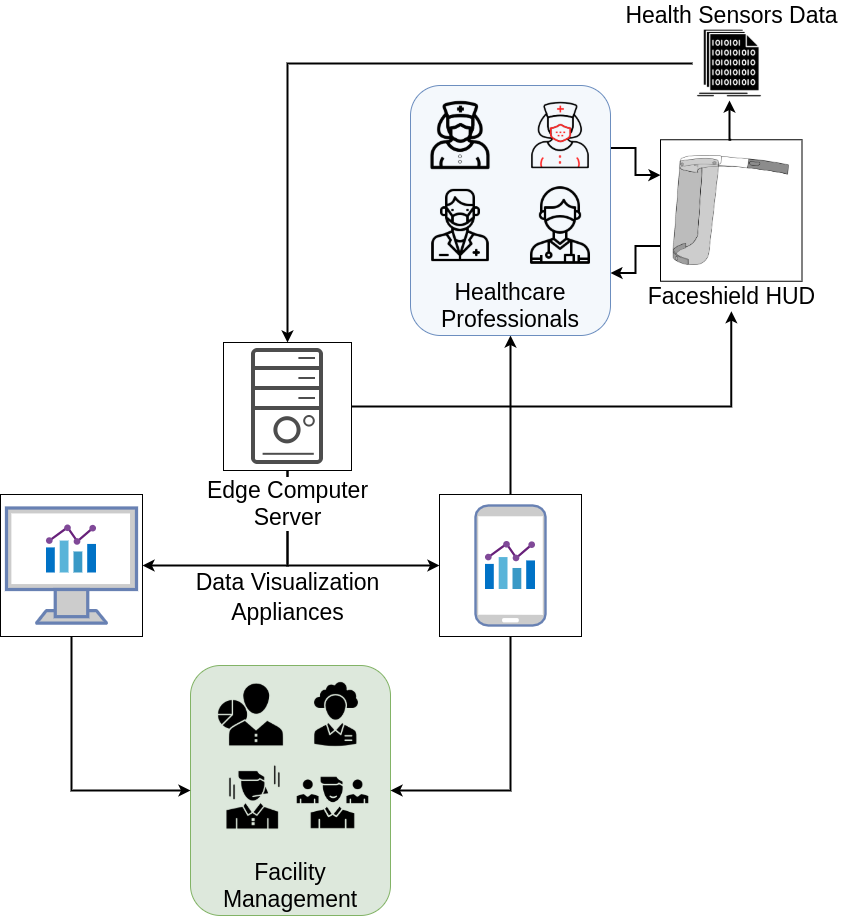
\includegraphics[width = .6\linewidth]{Figures/general-arch.png}
    \caption{Overview of the proposed architecture}
    \label{fig:gen-arch}
\end{figure}

The WLAN-server functions as a nearby edge computing facility that serves as an access point for wearable devices and computer connections. This module collects data from all the sensor nodes in the network, conducts processing activities to extract information and insights, and delivers high-level feedback through wearable, mobile, and computer terminal interfaces. This option enhances the capabilities of the Internet of Things appliances \cite{chang2017indie}, enabling to reach higher-level insights from the acquired data.

Health sensors, in this particular context, refer to wearable devices that are worn by healthcare practitioners. Our solution involves sensor nodes consisting of sensors connected to single-core computer-on-modules, which are powered by power banks. They carry out basic processing duties such as collecting data, preparing it for analysis, and facilitating two-way communication to transmit the collected information and receive responses. Medical practitioners and facilities administrators can utilize computer stations and mobile devices as interfaces as well.

\subsubsection{Edge Computing Devices Description}

\begin{figure}[h!]
    \centering
    %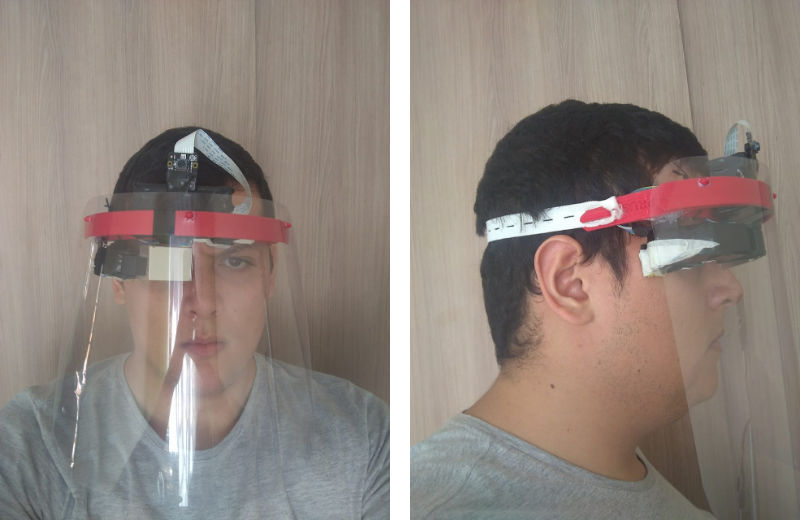
\includegraphics[width = .90\linewidth]{Figures/faceshield-proto.png}
    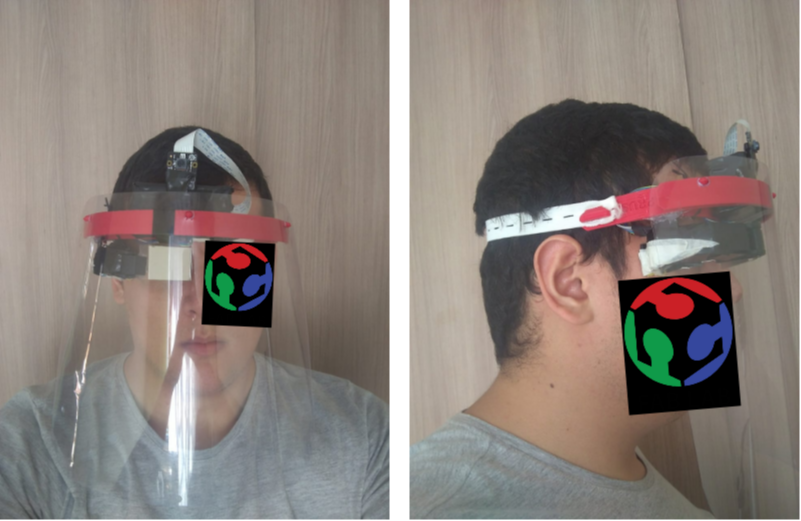
\includegraphics[width = .6\linewidth]{Figures/facecensor.png}
    \caption{Face shield HUD Prototype.}
    \label{fig:fsproto}
\end{figure}

We created a wearable gadget, specifically a prototype of the face shield HUD, for this project. We have already constructed and verified this prototype \cite{iceis21faceshield} as an obligatory safety apparatus in numerous healthcare establishments. The prototype that was created is shown in Figure \ref{fig:fsproto}.

The primary goal of this wearable gadget is to track and assess the user's health status and provide remote data retrieval. Using this device, we evaluate many aspects of the proposed solution. The primary pertinent part of the solution is the computer module. Wearable devices typically have limitations in terms of battery consumption and cost. Therefore, the initial choice is to utilize a solitary-core ARM-based computer-on-module as a foundation for creating the solution. A crucial component of the computer-on-module is a network board that has the capability to connect to a WLAN.

Another important aspect to take into account is the arrangement of the sensor. Historically, one of the primary advantages of wearable devices is enhancing the user's knowledge of their immediate surroundings and personal well-being \cite{majumder2017wearable}. This prototype is equipped with two distinct sensors. The first device is a pulse-oximeter and temperature sensor, which collects data on the user's health state. Another sensor present is a camera, which is used to gather data from the surrounding environment. 

Within the healthcare facility, the camera may retrieve data from patients' medical records by utilizing QR codes. Lastly, the feedback interface is the final part of it. In this regard, we have suggested the implementation of a head-up display (HUD) to furnish the user with comprehensive information. A Heads-Up Display (HUD) is an optically transparent display that presents information directly within the user's line of sight \cite{betancur2018research}. Augmented reality enhances usability and context awareness by allowing hands-free interaction and presenting information in the user's visual field.

\begin{figure}[h!]
    \centering
    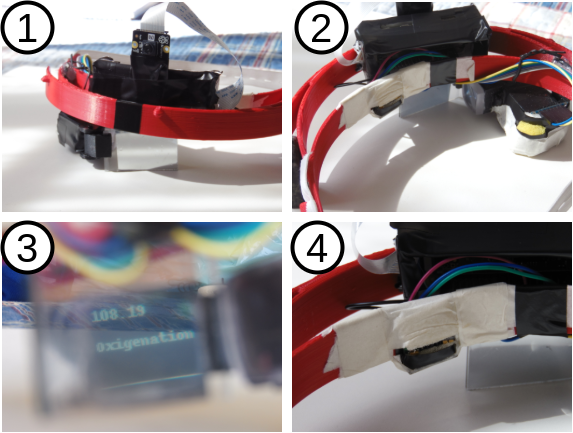
\includegraphics[width=.70\linewidth]{Figures/prototype-elements.png}
    \caption{Overview of the elements of the produced prototype}
    \label{fig:prt-elements}
\end{figure}

The prototype's elements are depicted in Figure \ref{fig:prt-elements}. In Figure 1, the primary mount is visible, featuring the camera positioned at the front and the HUD located below. In \textbf{2}, we can see the rearview, displaying the box containing the computer-on-module, the HUD system, and the monitoring sensors' location. Within \textbf{3}, the perspective from the HUD showcases an array of high-level data intended for the user's perusal. Ultimately, in \textbf{4}, the positioning of the health monitoring sensors and a portion of the wiring is visible.

\subsubsection{Terminal and Mobile Interfaces}

\begin{figure}[h!]
    \centering
    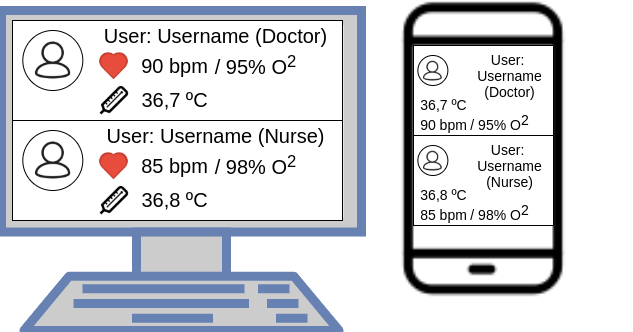
\includegraphics[width=.6\linewidth]{Figures/terminal-tools.png}
    \caption{Proposed Interfaces Illustration}
    \label{fig:interfaces}
\end{figure}

Another component of the suggested architecture is the management interfaces. These applications assist facility managers in the decision-making process. This technology facilitates the surveillance and identification of initial indications of pollution in healthcare practitioners \cite{doi:10.1111/acem.14053}. The instances of real-time monitoring of healthcare workers' situations are depicted in Figure \ref{fig:interfaces}.

\subsubsection{Edge Computer Server} 

\begin{figure}[h!]
    \centering
    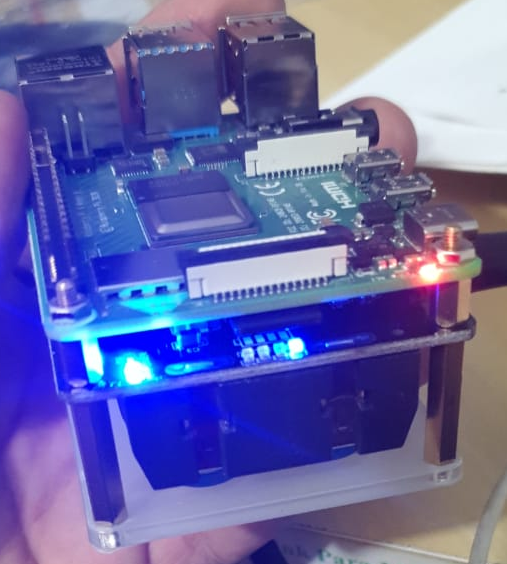
\includegraphics[width=.4\linewidth]{Figures/edge-server.png}
    \caption{Edge Computing Server Node}
    \label{fig:edgecomputer}
\end{figure}

The network edge consists of devices that manage computational operations in edge computing. The edge device must be engineered to efficiently handle such activities and meet requirements such as reliability. The integration of IoT components into the system occurs via an edge computer server. This device carries out two distinct functions inside this system. The initial component serves as a conduit for receiving, storing, and disseminating data from the wearable devices and the management terminal interfaces. The second objective is to input the obtained data into information extraction algorithms. In order to accomplish this goal, we suggested utilizing a portable device known as an edge computer server, which possesses the specified hardware prerequisites depicted in Figure \ref{fig:edgecomputer}. The depicted image showcases a Raspberry Pi4 model equipped with 4GB of RAM, 64GB of storage, and WiFi capabilities. The tests conducted with this gadget demonstrated a level of autonomy of approximately 12 hours under conditions of intensive usage.

\subsubsection{System Integration}

In order to comprehend the operation of this system, we moreover furnish an examination of the data flow. The diagram in Figure \ref{fig:dataflow} illustrates the key components of this architecture and depicts the flow of data. This depiction facilitates comprehension of the anticipated conduct of each constituent in accordance with its individual elements. Additionally, it is beneficial to analyze the temporal limitations associated with each stage of the procedure.

The suggested architecture consists of three distinct sorts of elements. The initial component is the wearable edge computing device, exemplified by the faceshield HUD. This component collects data from the sensors and performs initial processing to transform the data into meaningful information. 

The focal component is the Edge AI Computer/WLAN Server. This component serves as a central hub for data processing in an embedded edge computer, while also overseeing the network connections. In addition to serving as an access point on a computer, it is also capable of executing parallel data fusion and analysis activities. This method yields comprehensive data for the other components of the design. 
Lastly, the management interface serves as the final component in this arrangement. The generic interface block in Figure \ref{fig:dataflow} represents this element. Both mobile devices and computer terminals consist of essential components including user inputs, WLAN connectivity, processing, and output. 

\subsection{Experimental Tests}

A relevant aspect of distributed architectures is networking performance. This feature directly affects the quality of the provided services in IoT-based systems, having consequences in the system's real-time capabilities \cite{cao2018qos}. Thus, the experimental setup evaluates the timing constraints for the data flow and processing.

\subsubsection{Real-Time as Quality-of-Service}

To evaluate these aspects, we perform a QoS-based timing constraint test. The experiment was designed as a QoS formalization, presented on similar studies concerning IoT and Wireless Sensor Networks \cite{silva2019analyzing} to evaluate soft real-time constraints as network timing constraints.

At first, we divide the experiment time in discrete intervals, as the set $T = t_i,  i \in \mathbb{N}$, where $t_{i+1} - t_i = \theta$, where $\theta$ is a constant sampling time. The soft real-time deadline will be represented by $\phi$, where $\phi = k \times \theta, k \in \mathbb{N}^*$. From these primary statements, we establish the following definitions:

\begin{definition} 
    Let $D = d_i$ be the finite set of nodes consuming and producing data from the middleware node, where $i \in \mathbb{N}$;
\end{definition}

\begin{definition}
    Let $E = e_i$ be the finite set of events that each node performs, where $i \in \mathbb{N}$;
\end{definition}

\begin{definition}
    Let $L = l_{d,e}$ be the length of time interval that the node $d$ takes to perform an event $e$, where $d \in D$ and $e \in E$;
\end{definition}

\begin{definition}
    Let $P = p_{i}$ be the set of patterns of events to be observed in the devices, where $p_i = E_i$, $E_i \subset E$ and $i \in \mathbb{N}$;
\end{definition}

\begin{definition}
    Let $O = o_{i}$ be the finite set of observations of a certain pattern $p_i \in P$ on the devices;
\end{definition}

The equation that represents the elapsed time $\lambda$ to observe a particular pattern $p_i \in P$ is:

\begin{equation}
    \lambda_{o_i} = \sum l_{d,e_k} | \forall e_k \in o_i, o_i = O_{p_i}
\vspace{0.2cm}
\end{equation}

In this case, each device in the network composition can have its single $\phi_i$ soft real-time deadline. Given this equation, let $\hat{O}$ be a subset of $O$, where $\lambda_{o_i} \leq \phi_i$, $\forall o_i \in \hat{O}$. Finally, given the sets $O$ and $\hat{O}$:

\begin{definition}
    Let $N$ be the number of elements on the set $O$;
\end{definition}

\begin{definition}
    Let $N_h$ be the number of elements on the subset $\hat{O}$;
\end{definition}

The following equation will represent the quality factor $Q_f$:

\begin{equation}
    Q_f = \frac{N_h}{N} (\times 100 \%)\\
    \vspace{0.2cm}
\end{equation}

The nodes will try to gather or update data from the server node in parallel on each test. This result represents how often the nodes execute a pattern of events without violating the soft real-time constraints. This perspective allows experimenting on how increasing the number of devices producing and consuming data affects the network quality factor.

The proposed experiment is divided in 3 stages:

\begin{itemize}
    \item \textbf{Stage 1:} Defining the soft real-time constraint;
    \item \textbf{Stage 2:} Evaluating the effect of stressing the system by increasing the number of edge devices;
    \item \textbf{Stage 3:} Evaluating the effect of stressing the system by increasing the number of client interfaces.
\end{itemize}

During \textbf{Stage 1}, we execute a simplified version of the appliance, which includes a single element from each class depicted in Figure \ref{fig:dataflow}. To determine the minimum $\phi_i$ soft real-time constraint, we utilize the provided data to achieve a quality factor of 0.95 (95\%). This limitation will serve as a benchmark for assessing the system's performance while scaling up the number of devices, with a block length of $\theta = 2$ ms. Furthermore, we utilize this data to assess the intrinsic timing restrictions of each device for the purpose of simulation.

During \textbf{Stage 2}, we utilize the limitations established in the initial stage to assess the performance of the system as the quantity of edge devices is augmented. The computer-on-module boards will be utilized to replicate the behavior of various devices, as done in the production of the prototype. The timing for each job on the simulated device is derived from the assessment conducted in the previous stage.

In \textbf{Stage 3}, we assess the impact of increasing the quantity of terminal interfaces. To address this issue, we create many simulated terminals as separate processes on a machine that is linked to the network.

These stages serve as a means of validating the proposed architecture and providing an overview of the limitations when it comes to scaling up the number of devices and customers in this system.

\subsubsection{Server Behavior Evaluation}

For the second experiment, we consider the influence of patients and medical professionals in the environment. Also, in this case, we evaluate the timing aspect. We evaluate how the overload of patients and medical devices in the network influence the server capability of answering requests. For this matter, we consider the dataflow presented in Figure \ref{fig:xpsetup}.

\begin{figure}[h!]
    \centering
    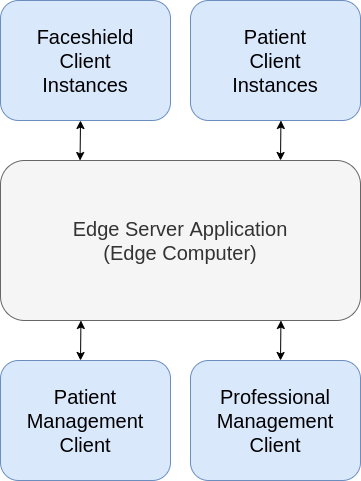
\includegraphics[width = .35\linewidth]{Figures/experimental-setup.png}    \caption{Data Flow for the Experimental Setup on the Second Test}
    \label{fig:xpsetup}
\end{figure}

In this instance, we replicated the actions of numerous customers that generated and utilized data from the edge server. The patient appliance is regarded as a sensor for measuring temperature and pulse-oximeter readings, and it has the same temporal constraints as in the previous stage.

From this standpoint, the solution has five distinct groups of elements. The primary and pivotal component is the edge computing server. The system operates an application that receives connections from several customers, storing their data and providing it for requests from management apps in the wireless local area network. The management clients consist of the second and third aspects. The patient management client retrieves data from a specific patient by using their name as an identifier. The key worker management client collects data from all professionals employed at the facility. Ultimately, the fourth and fifth aspects represent the occurrences specifically tailored for clients in the healthcare device industry. They operate in a similar manner, as they both necessitate data collection from identical sensors.

In order to assess the efficacy of this system within the network, we conducted an analysis of two distinct situations. Initially, we augmented the quantity of instances for the face shield device from 5 to 50, while maintaining a consistent count of 20 patient instances. Next, we conducted a second test scenario in which we augmented the quantity of patient device instances from 5 to 50, while maintaining a consistent number of 20 face shield device instances. In all cases, we ran one instance of the patient management client and another instance of the key workers' management client.

The parameter for this response is the server's response time, which is measured throughout the entire execution. In this regard, we assessed the mean response time and the rolling average during program execution. We conducted both tests for around 600 seconds, modifying the payload on the variable that induces stress in the test every 60 seconds.


\subsection{Results}

\subsubsection{Devices Internal Constraints Evaluation}

Firstly, we assess the inherent timing restrictions of the device. This stage represents the initial phase in establishing a validation environment that closely replicates the conditions encountered in real-world scenarios. In this context, we provide a description of both the server apps and the clients, which include terminal and wearable devices. Furthermore, we empirically ascertain the temporal limitations in the prototype in order to establish authentic simulation environments.

Let us begin by discussing the server program. The server stores the latest data from all the clients in its memory for the experimental group, and then transmits the entire information to the asking terminal clients. Additionally, the server monitors the temporal limitations for experimental reasons. 

In order to facilitate the connecting of several clients, we have created a server that utilizes multiple threads. Each thread is tasked with managing a solitary client. The application utilizes two essential processes: capturing the most recent health data from each wearable client and recording it in the log file's handler. The algorithm executed by each thread managing a single client connection is illustrated in Figure \ref{fig:server-algorithm}. The crucial sessions are highlighted in red blocks.

\begin{figure}[h!]
    \centering
    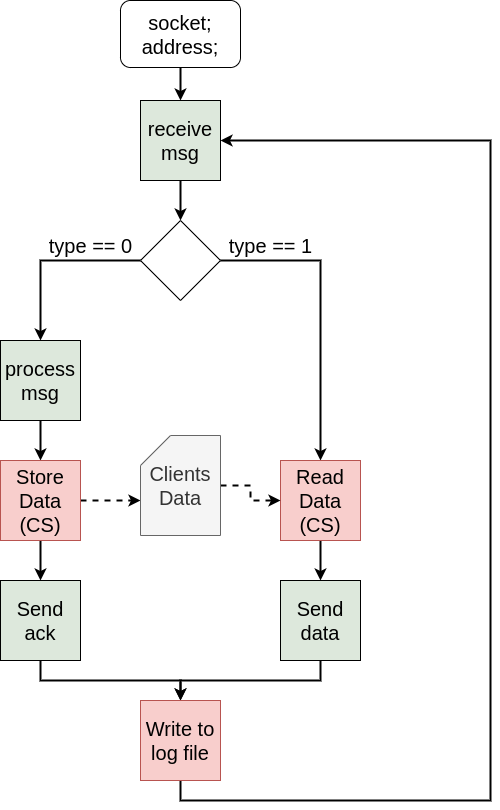
\includegraphics[width = .4\linewidth]{Figures/server-algorithm.png}
    \caption{Edge Server Node Algorithm}
    \label{fig:server-algorithm}
\end{figure}

The processes commence with the handlers responsible for the creation of connections and information management. The client address and port information serve as indices for the client data stored in memory. This device caters to two categories of users: terminal clients and wearable clients. Messages of terminal requests are identified by ``type == 1'', and messages from the wearable clients are identified by ``type == 0''. 

The threads store the customers' information in a unified data structure. Hence, the initial crucial segment involves engaging in reading and writing inside this framework. The data received from the clients is analyzed and kept. Terminals receive data from all available clients in response to requests. Ultimately, the threads utilize the identical log file. Therefore, it is likewise a second crucial segment.

\begin{figure}[h!]
    \centering
    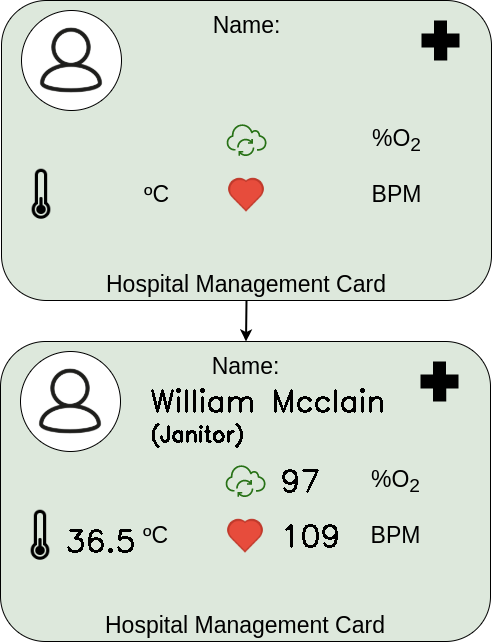
\includegraphics[width = .4\linewidth]{Figures/card-gen.png}
    \caption{Visualization Prototype Application Example}
    \label{fig:card-gen}
\end{figure}

The initial type of client is the terminal client. This client consists of two primary stages: (i) retrieving data from the server, and (ii) processing the data and presenting it on a screen using a background template and the collected information. The background and an example of a card made using simulated information are depicted in Figure \ref{fig:card-gen}. Ultimately, the threads utilize the identical log file. Therefore, it is likewise a second crucial segment.

The wearable client is responsible for three distinct tasks: (i) retrieving data from the sensors, (ii) transmitting data to the server and receiving the server's response, and (iii) analyzing the data and presenting a visual representation on the OLED display. Tasks (i) and (iii) are internal, however task (ii) relies on network connectivity. In order to ascertain the necessary timing specifications for executing this application, we conducted tasks (i) and (iii) on the prototype depicted in Figure \ref{fig:fsproto} for a duration of 120 seconds, while monitoring the durations required to complete both internal operations. The results obtained, on average, show that:

\begin{itemize}
    \item Task (i) takes an average time of 2.25 $\pm$ 0.10 ms;
    \item Task (iii) takes an average time of 11.8 $\pm$ 14.3 ms.
\end{itemize}

With this data, we created an application to emulate the client's behavior for the stress tests (Stages 2 and 3). The prototype also uses the application to determine the real-time constraint in Stage 1. 

\subsubsection{Stage 1: Real-Time Constraints Definition}

In order to establish the real-time limitations, we assess the timing specifications of the tasks executed by each device inside the framework of this test. In this case, we utilize the definition of the quality factor. In this stage, we assess the basic setup by running only one piece from each class on the desired hardware. The server operates on a Raspberry Pi 3 Model B, the interface operates on a desktop computer, and the wearable application operates on an embedded Raspberry Pi Zero W, which is attached to the prototype face shield.

During the initial phase, our objective is to determine the soft real-time constraint $\phi$. The experiment period is partitioned into discrete-time intervals of $\theta=$ 2 ms. To address this issue, we set a desired quality factor of $Qf = 0.95$. Next, we determine the minimal number of time blocks required to meet the desired restriction, which is a multiple of the number of blocks $k$ needed to achieve the desired aim. For every class of device, we define a distinct limitation that corresponds to its specific set of functions. 

\begin{table}[h!]
\centering
\caption{Real Time Constraint Definition Results}
\label{tab:rt-def}
\begin{tabular}{lll}
\hline
 & Average time (ms) & Requirement ($k$) \\ \hline
\multicolumn{1}{l}{WEARABLE} & 27.6 $\pm$ 27.4 & 37 blocks \\ %\hline
\multicolumn{1}{l}{INTERFACE} & 27.7 $\pm$ 33.3 & 33 blocks \\ %\hline
\multicolumn{1}{l}{SERVER} & 54.4 $\pm$ 50.4 & 65 blocks \\ \hline
\end{tabular}
\end{table}

In the subsequent phases, we employ the limitations outlined in Table \ref{tab:rt-def} to assess the impact of exerting additional pressure on the system through an increased number of clients and interfaces. The stress tests are still being conducted on the Raspberry Pi 3 Model B server. The interface appliance is operated by one computer, while another computer executes many instances of simulated client applications.

\subsubsection{Stage 2: Stressing the System with more Wearable Edge Devices}

The primary goal of the initial test is to ascertain the impact of augmenting the quantity of wearable gadgets on network efficiency. We executed a range of 5 to 50 instances of the program that simulates the behavior of a wearable device on the network for the purpose of this test. Throughout the entire duration of the test, we ran a solitary interface application.

Initially, we derived the aggregate values for the quality factor based on the fixed elements. Based on our comprehensive testing during the entire duration, the results consistently indicate that:

\begin{itemize}
    \item The quality factor for the interface was $Q_f = 0.989$;
    \item The quality factor for the server was $Q_f = 0.937$;
\end{itemize}

\begin{figure}[h!]
    \centering
    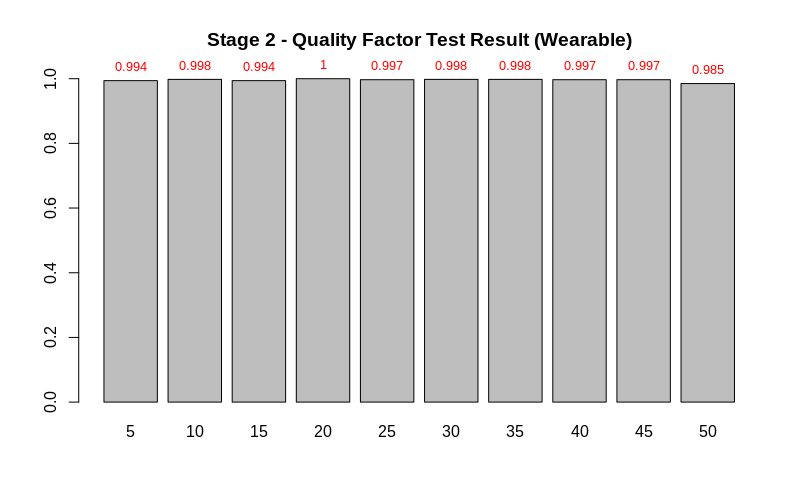
\includegraphics[width=.7\linewidth]{Figures/qf-s2.png}
    \caption{Quality Factor Test Results}
    \label{fig:qf-s2}
\end{figure}

The findings for the quality factor test are shown in Figure \ref{fig:qf-s2}. The degradation in quality observed when scaling up the system was approximately 1\%. This phenomenon demonstrates that the system design is capable of collecting and controlling data from different devices without violating the soft real-time limitation. In addition, the other limitations encountered a minimal level of compromise, so reinforcing this initial finding.

\subsubsection{Stage 3: Stressing the System with more Terminal Devices}

The purpose of this test is to examine the performance of data-intensive applications in conditions of concurrent stress. For this instance, we altered the quantity of emulated terminal devices. The terminal devices collect data from all connected clients for the management applications. We ran the application multiple times, ranging from 5 to 50 instances. Throughout the duration of the test, we simulated 20 wearable devices.

Initially, we derived the aggregate values for the quality factor based on the fixed elements. Based on our comprehensive testing during the entire duration, the results consistently indicate that:

\begin{itemize}
    \item The quality factor for the wearable devices was $Q_f = 0.986 \pm 0.001$;
    \item The quality factor for the server was $Q_f = 0.885$;
\end{itemize}

\begin{figure}[h!]
    \centering
    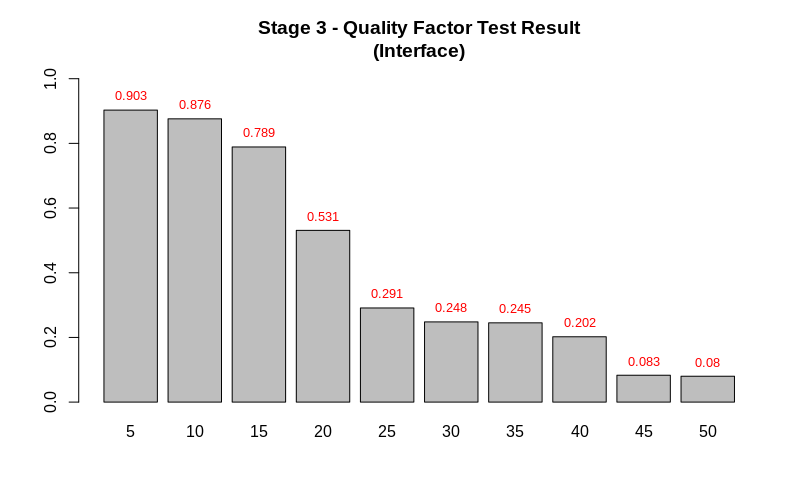
\includegraphics[width=.7\linewidth]{Figures/qf-s3.png}
    \caption{Quality Factor Test Results}
    \label{fig:qf-s3}
\end{figure}

The findings for the quality factor test are shown in Figure \ref{fig:qf-s3}. Expanding the quantity of instances in this scenario greatly undermines the real-time capability of this program. This trend is reinforced by the deterioration in the quality factor on the server. This outcome suggests that it is preferable to do extensive data processing on the edge server whenever feasible, as transmitting substantial data quantities can compromise the reliability of the architecture.

\subsubsection{Server Behavior Evaluation}

\begin{figure}[h!]
    \centering
    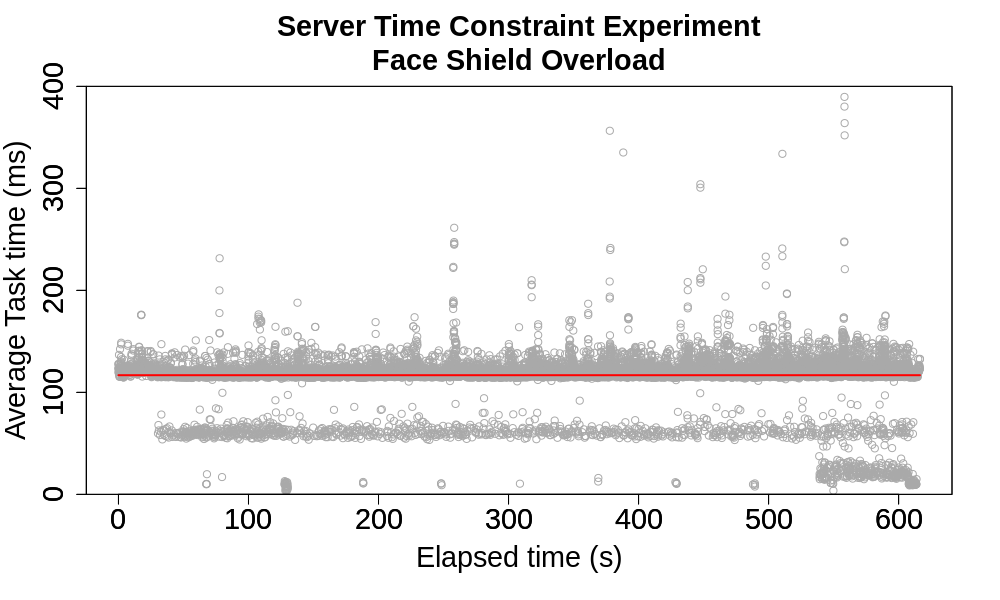
\includegraphics[width = .7\linewidth]{Figures/server-t1-times.png}
    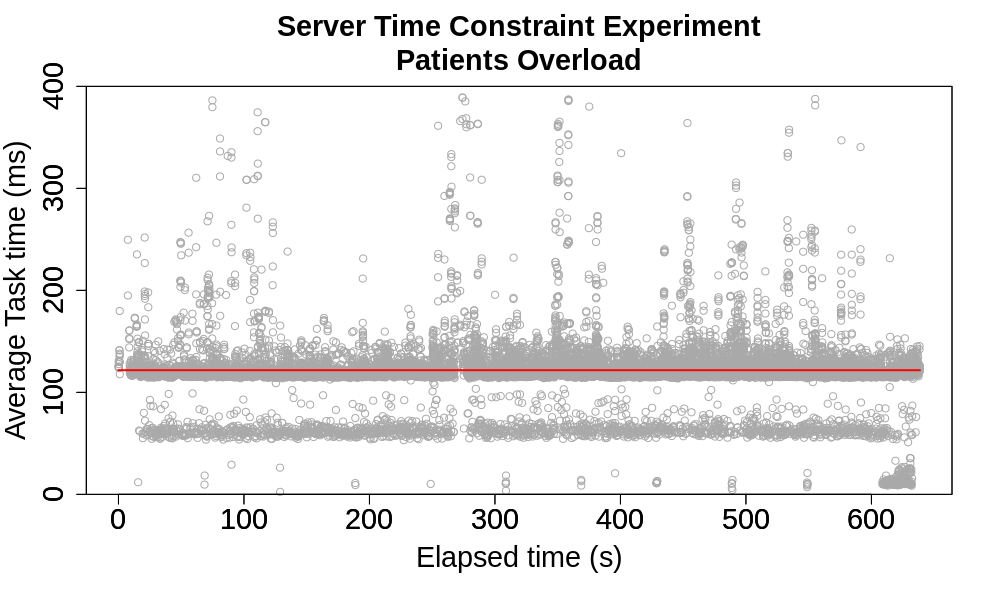
\includegraphics[width = .7\linewidth]{Figures/server-t2-times.png}
    \caption{Performance Test Results}
    \label{fig:test-results}
\end{figure}

This final test assesses the impact of client overload on the system's performance. The findings obtained for the testing are shown in Figure \ref{fig:test-results}. The moving average results during the test are shown in gray. The red line represents the mean duration for the system to handle a request and transmit the outcome.

We calculated a moving average by averaging 100 consecutive samples for both tests. The average response time for a single sample in the initial test was $116.9 \pm 19.11$ milliseconds. The moving average indicates that the mean time is rather stable during the execution, with a few exceptional numbers. The initial outcome demonstrates the system's stability, even under increased device load. The second test yielded an average time limitation of $121.8 \pm 73.28$ ms. While the moving average generally indicates a similar pattern to the first test, with stability around the global average, it also identifies more outlier values, indicating a larger standard deviation.

\section{Wearable-based human activity recognition}

Within this section, we will introduce the suggested framework and its various components. Initially, it is imperative to comprehend the equipment implicated in the project. Furthermore, it is crucial in this solution to comprehend the integration process and the algorithm accountable for forecasting the actions. Our proposal involves utilizing a minimalist wearable device and a recurrent neural network (namely, LSTM) to carry out the classification task. Ultimately, we assess the incorporation of cloudlets and mobile edge computing.


\subsection{Requirements}

To begin this study, it is necessary to assess the prerequisites for the proposed approach. To address this issue, we provide a modified version of the co-design diagram shown in Figure \ref{fig:simplified-codesign-6}, which is a simplified rendition of the diagram depicted in Figure \ref{fig:codesign-2.0}.

\begin{figure}[ht!]
    \centering
    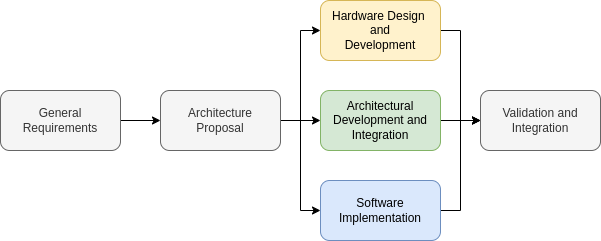
\includegraphics[width = .8\linewidth]{Figures/simplified-codesign.png}
    \caption{Simplified Co-design diagram.}
    \label{fig:simplified-codesign-6}
\end{figure}

This representation displays the need to raise the constraints for the application and classify them into the hardware, software or architectural domain. The constraints identified for this matter are:

\begin{itemize}
    \item This solution must gather data from the users with small scale sensors [\textit{Hardware}].
    \item The wearable devices must have low current consumption for an increased autonomy [\textit{Hardware}].
    \item The integration of data from multiple devices must happen within and edge server [\textit{Architecture}].
    \item The communication needs to be efficient to stream the data through this local network [\textit{Architecture}].
    \item Data obtained from the applications must be processed in real-time [\textit{Software}].
\end{itemize}

This solution shares comparable limitations with the preceding options. In this instance, we suggested incorporating small-scale wearable devices with microcontroller units (MCUs) that have wireless capabilities. We suggested employing recurrent neural networks with a wearable server to carry out the specified task.

\subsubsection{Edge Computing Architecture}

The architecture of edge computing consists of two primary levels. Within the initial stratum, uniform wearable gadgets generate data from individual users. The second layer is equipped with an edge server that receives data from the sensors, forecasts the current activity, and stores it in a database. Figure \ref{fig:layers} depicts the layers of the proposed architecture. 

\begin{figure}[h!]
    \centering
    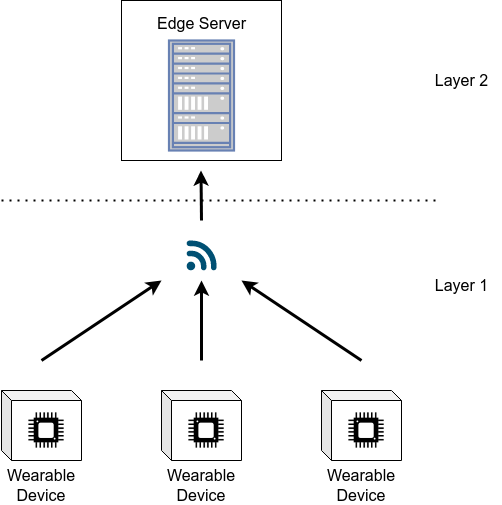
\includegraphics[width = .45\linewidth]{Figures/layers.png}
    \caption{Architecture layers}
    \label{fig:layers}
\end{figure}

The wearable gadget in this design possesses a straightforward configuration. The processing unit is a microcontroller (MCU) with the ability to communicate wirelessly using Wi-Fi (IEEE 802.11). This choice is made to ensure minimal processing power requirements throughout the development of this gadget. The sensor of the device consists of a solitary 6-DoF IMU. The proposed system is powered by a battery, serving as the final component in this idea. The schematic model of the proposed solution is depicted in Figure \ref{fig:wearable}.

\begin{figure}[h!]
    \centering
    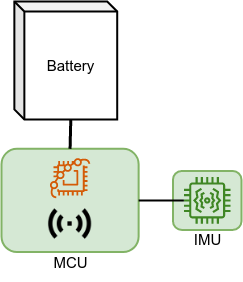
\includegraphics[width = 0.3\linewidth]{Figures/wearable.png}
    \caption{Wearable device schematics proposal}
    \label{fig:wearable}
\end{figure}

For the second layer, we suggest employing an edge server to execute the Edge AI algorithm. In this regard, we conducted experiments from two different viewpoints. One approach involves utilizing a cloudlet architecture to carry out this task. In this study, we conducted tests on the algorithm utilizing a desktop computer equipped with a six-core i5-9600K CPU running at a speed of 3.70GHz, an RTX 2060 super GPU, and 32GB of RAM. We conducted tests on a mobile edge platform equipped with a quad-core ARM A57 processor running at 1.43 GHz, a 128-core Maxwell GPU, and 4GB of memory. The mobile edge platform utilized in this experiment is depicted in Figure \ref{fig:jetson}.

\begin{figure}[h!]
    \centering
    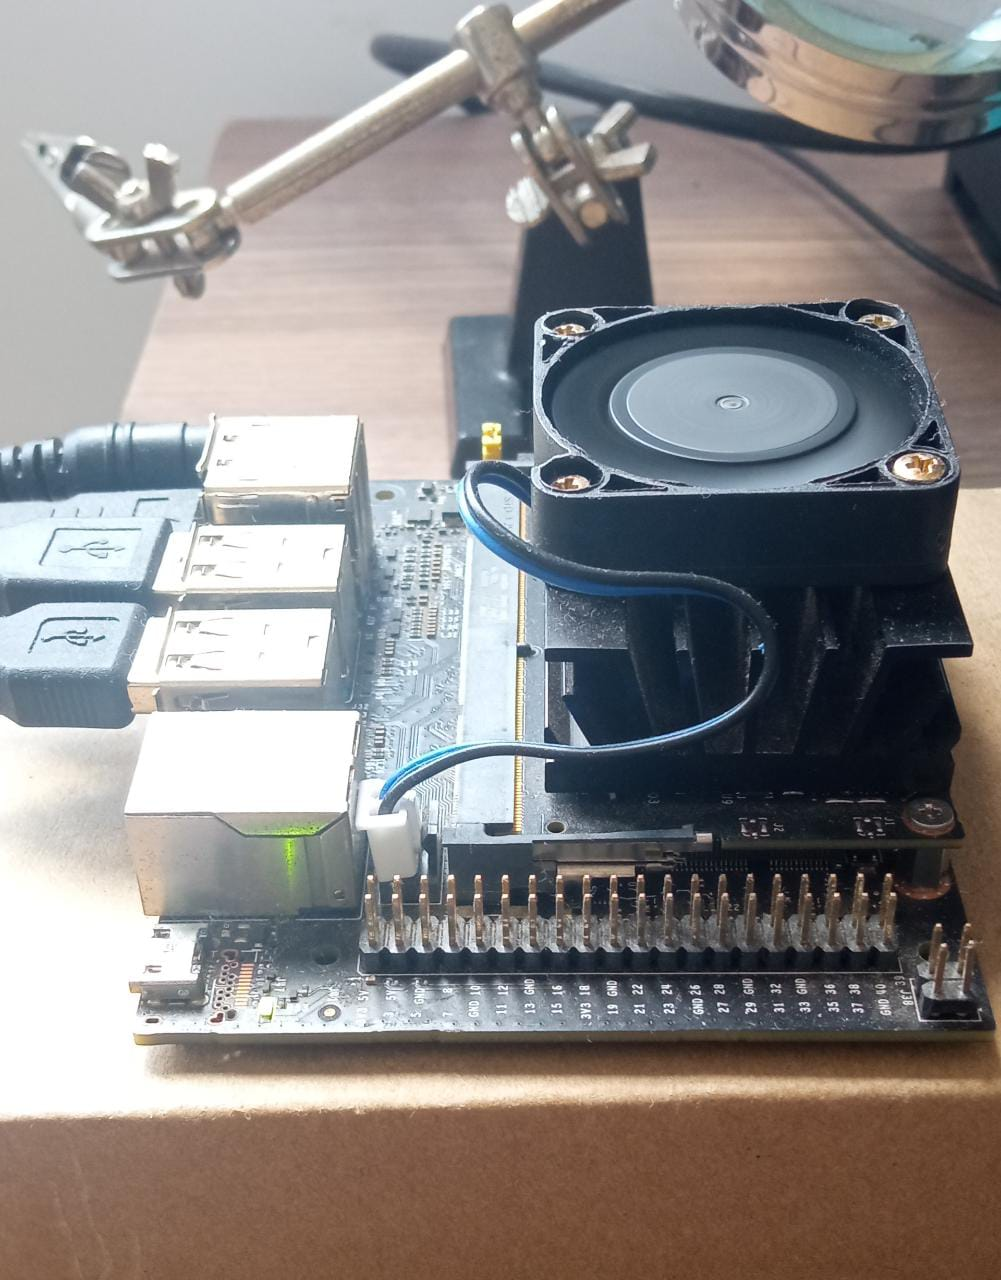
\includegraphics[width = .4\linewidth]{Figures/jetson.jpeg}
    \caption{Mobile edge computing platform}
    \label{fig:jetson}
\end{figure}

Considering this proposed architecture and experimental setup, we evaluated the usage of a recurrent neural network exploring a theoretical data generation using data from a public dataset. Furthermore, we evaluate the temporal constraints for each edge server setup.

\subsubsection{AI Model Proposal and Training}

The gathered data consists of a collection of time series obtained from the sensors. For this particular scenario, we employ a Long Short-Term Memory (LSTM) model to forecast the behavior based on a collection of unprocessed time series data. Therefore, we opted for a recurrent neural network design to forecast the actions.

The first stage involved selecting a publicly available dataset that possessed similar characteristics to the required dataset. We used the KU-HAR dataset \cite{sikder2021ku} as our initial foundation. The dataset comprises samples from 18 distinct activities executed by a total of 90 people. The authors modified the data to achieve a sampling rate of 100 Hz, which serves as a foundation for developing the MCU-based wearable device. The data was partitioned using a sliding window of two seconds, with a half-second overlap. 90\% of the data was allocated for training, while 5\% each was allocated for validation and testing. Ultimately, the training set consisted of 108976 samples, the validation set contained 6111 samples, and the test set comprised 8313 samples. The table labeled as "Table \ref{tab:classes}" presents the collection of jobs outlined in this dataset.


% Please add the following required packages to your document preamble:
% \usepackage{graphicx}
\begin{table}[h!]
\centering
\caption{Classes of activities in the KU-HAR dataset}
\label{tab:classes}
\resizebox{.25\linewidth}{!}{%
\begin{tabular}{ll}
\hline
\textbf{Label} & \textbf{Activity} \\ \hline
0 & Stand \\
1 & Sit \\
2 & Talk-sit \\
3 & Talk-stand \\
4 & Stand-sit \\
5 & Lay \\
6 & Lay-stand \\
7 & Pick \\
8 & Jump \\
9 & Push-up \\
10 & Sit-up \\
11 & Walk \\
12 & Walk-backwards \\
13 & Walk-circle \\
14 & Run \\
15 & Stair-up \\
16 & Stair-down \\
17 & Table-tennis \\ \hline
\end{tabular}%
}
\end{table}

We propose using a network with 128 LSTM cells in the first layer. Then the next layer is a dense neural layer with 256 neurons. Finally, the output has 18 layers with the ``softmax'' activation function, configuring a generative classification model. This classification results from the output that generates the highest probability. Figure \ref{fig:lstm} illustrates the proposed architecture.

\begin{figure}[h!]
    \centering
    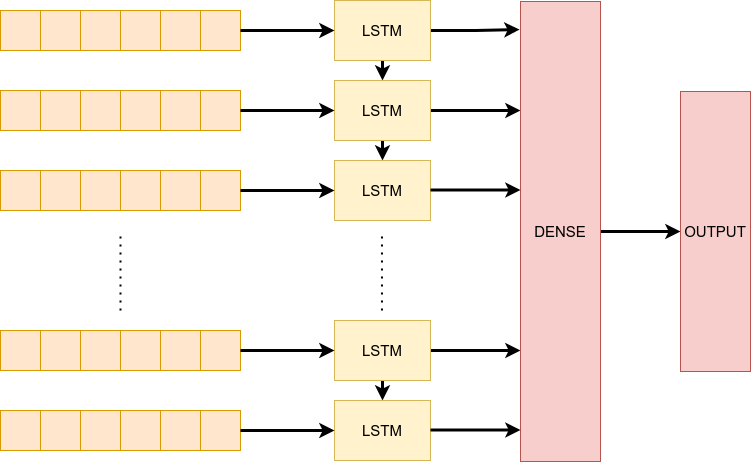
\includegraphics[width=.7\linewidth]{Figures/lstm.png}
    \caption{LSTM illustration}
    \label{fig:lstm}
\end{figure}

The loss function was categorical cross-entropy. We trained the algorithm until the loss convergence. We configure the convergence condition as no improvement higher than 0.0001 for 15 epochs of training. We also reduced the learning rate as the model reached 4-epoch-plateaus. Figure \ref{fig:training} displays the graphs for loss and global accuracy during the training process.

\begin{figure}[h!]
    \centering
    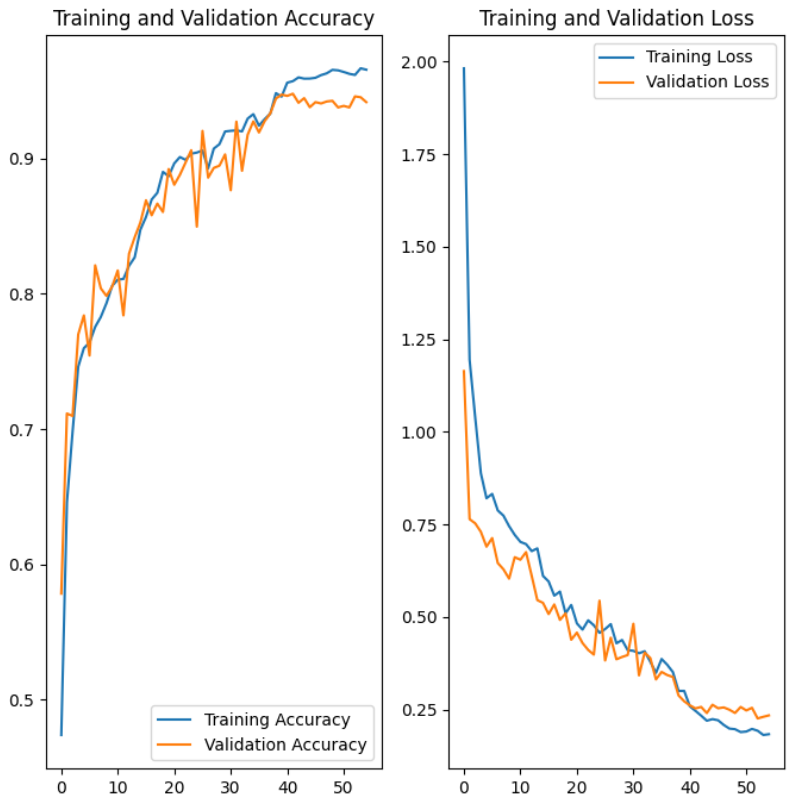
\includegraphics[width=.5\linewidth]{Figures/training.png}
    \caption{Training session result}
    \label{fig:training}
\end{figure}

Finally, we converted the model to the ``tflite'' format for embedding and testing. After defining the edge computing architecture, proposing the algorithm, and performing its training, the next step is establishing evaluation tools and metrics to understand the performance of the proposed system.

\subsection{Evaluation Tests}

With the previously established proposal of an edge computing architecture and training of the proposed algorithm, we require the definition of tests and metrics to evaluate the experimental aspects of this work. Initially, we propose a set of metrics based on usual multi-class classification tasks. Then we propose evaluating the proposed solution's timing aspects in the cloudlet and mobile edge sets.

\subsubsection{Algorithm Evaluation}

The problem stated in this case is a multi-class classification. To evaluate the model, we initially employ the most traditional multi-class classification metrics for AI. These metrics are \textit{precision} ($P_c$), \textit{recall} ($R_c$) and \textit{F1-Score} ($F1_c$), calculated for each class $c$ and defined by:

\begin{equation}
    P_c = \frac{TP_c}{TP_c+FP_c},
\end{equation}

\begin{equation}
    R_c = \frac{TP_c}{TP_c+FN_c},
\end{equation}

\begin{equation}
    F1_c = 2 \times \frac{P_c \times R_c}{P_c + R_c}.
\end{equation}

These equations depend on the variables $TP_c$ (true positives for each class $c$), $FP_c$ (false positives for each class $c$), and $FN_c$ (false negatives for the class $c$). We also evaluate the global accuracy $A_g$, which can be calculated by the two forms below with the same result:

\begin{equation}
    A_g = \frac{TP}{TP + FN},
\end{equation}

or

\begin{equation}
    A_g = \frac{TP}{TP + FP}.
\end{equation}

In these equations, the variables $TP$, $FN$, and $FP$ are the sums of the variables they represent for each class, as displayed:

\begin{equation}
    TP = \sum_c TP_c,
\end{equation}

\begin{equation}
    FP = \sum_c FP_c,
\end{equation}

\begin{equation}
    FN = \sum_c FN_c.
\end{equation}

These metrics help to understand the quality of the model's predictions. In the next stage, we also evaluate timing constraints regarding the two edge computing perspectives. 


\subsubsection{Architecture Evaluation}

Given an algorithm employing a solitary-queue prediction pipeline, it is necessary for each user to receive a prediction from the system every 0.5 seconds. If the worst-case situation occurs, the device will be faced with a complete queue that needs to be resolved within a 0.5 second timeframe. This formulation indicates the maximum number of devices that the edge server can process in an asymptotic limit. In relation to this issue, we assess the asymptotic limit in the following manner:

\begin{equation}
\label{eq:limit}
    L_t = \frac{0.5}{\mu_t+2\sigma}
\end{equation}

In this context, $L_t$ represents the ultimate number of users that the edge server can handle, $\mu_t$ denotes the average duration required for each prediction, and $\sigma$ represents the variability in the prediction timings. The function is intended to encompass approximately 90\% of the situations, taking into account the $2\sigma$ factor. The limit is a theoretical limitation of the system, which is based on a soft real-time constraint. It does not take outliers into account as critical circumstances. We also assess the timing restrictions in a qualitative manner using the obtained data.

\subsection{Results and Discussion}

The next part provides the outcomes acquired from the conducted experiments. At first, we evaluated the algorithm based on the predetermined metrics. Next, we assess the theoretical temporal limitations. Lastly, we will analyze the acquired outcomes and their consequences.

\subsubsection{Algorithm Evaluation}

In Figure \ref{fig:training} from the corresponding section, we presented the outcomes obtained after training the algorithm. The graphs suggest that the training procedure occurred without overfitting, based on qualitative analysis. Therefore, we assess the specified indicators at this point. 

We conducted an initial assessment of the data obtained from the validation set. The results collected in this test are displayed in Table \ref{tab:metrics-validation}. The program achieved an accuracy rate of over 90\% in correctly identifying the appropriate classification across most categories. Under the most unfavorable circumstances for this test, the algorithm achieved a prediction accuracy of 79\%. The overall precision rate reached 94.7\% on a worldwide scale. The results shown here surpass the initial findings reported by the dataset authors \cite{sikder2021ku} (84.7\%) and another study that references the work of Abid and Nahid \cite{abid2021two} (89.5\%). These findings demonstrate that this method is capable of performing the specified task to a significant degree. The findings collected in this step are displayed in Figure \ref{fig:cfmat-val} and Table \ref{tab:metrics-validation}.


\begin{table}[h!]
\centering
\caption{Classification Metrics for the Validation Set}
\label{tab:metrics-validation}
\resizebox{.7\linewidth}{!}{%
\begin{tabular}{lllll}
\hline
\textbf{Activity} & \textbf{Precision} & \textbf{Recall} & \textbf{F1-Score} & \textbf{Support} \\ \hline
Stand & 0.95 & 0.94 & 0.94 & 617 \\
Sit & 0.90 & 0.96 & 0.93 & 619 \\
Talk-sit & 0.93 & 0.88 & 0.91 & 499 \\
Talk-stand & 0.92 & 0.99 & 0.95 & 478 \\
Stand-sit & 0.98 & 0.99 & 0.99 & 657 \\
Lay & 0.99 & 0.97 & 0.98 & 477 \\
Lay-stand & 0.95 & 0.95 & 0.95 & 443 \\
Pick & 0.97 & 0.90 & 0.93 & 383 \\
Jump & 0.99 & 1.00 & 0.99 & 158 \\
Push-up & 1.00 & 0.92 & 0.96 & 151 \\
Sit-up & 0.99 & 0.98 & 0.99 & 449 \\
Walk & 0.92 & 1.00 & 0.96 & 235 \\
Walk-backwards & 0.94 & 0.92 & 0.93 & 130 \\
Walk-circle & 0.85 & 0.95 & 0.90 & 81 \\
Run & 0.80 & 0.95 & 0.87 & 84 \\
Stair-up & 0.92 & 0.79 & 0.85 & 278 \\
Stair-down & 0.95 & 0.94 & 0.95 & 249 \\
Table-tennis & 0.97 & 0.97 & 0.97 & 123 \\ \hline
Macro Avg. & 0.94 & 0.94 & 0.94 & 6111 \\
Weighted Avg. & 0.95 & 0.95 & 0.95 & 6111 \\ \hline
Global accuracy: & \multicolumn{4}{l}{94.7 \%} \\ \hline
\end{tabular}%
}
\end{table}

\begin{figure}[h!]
    \centering
    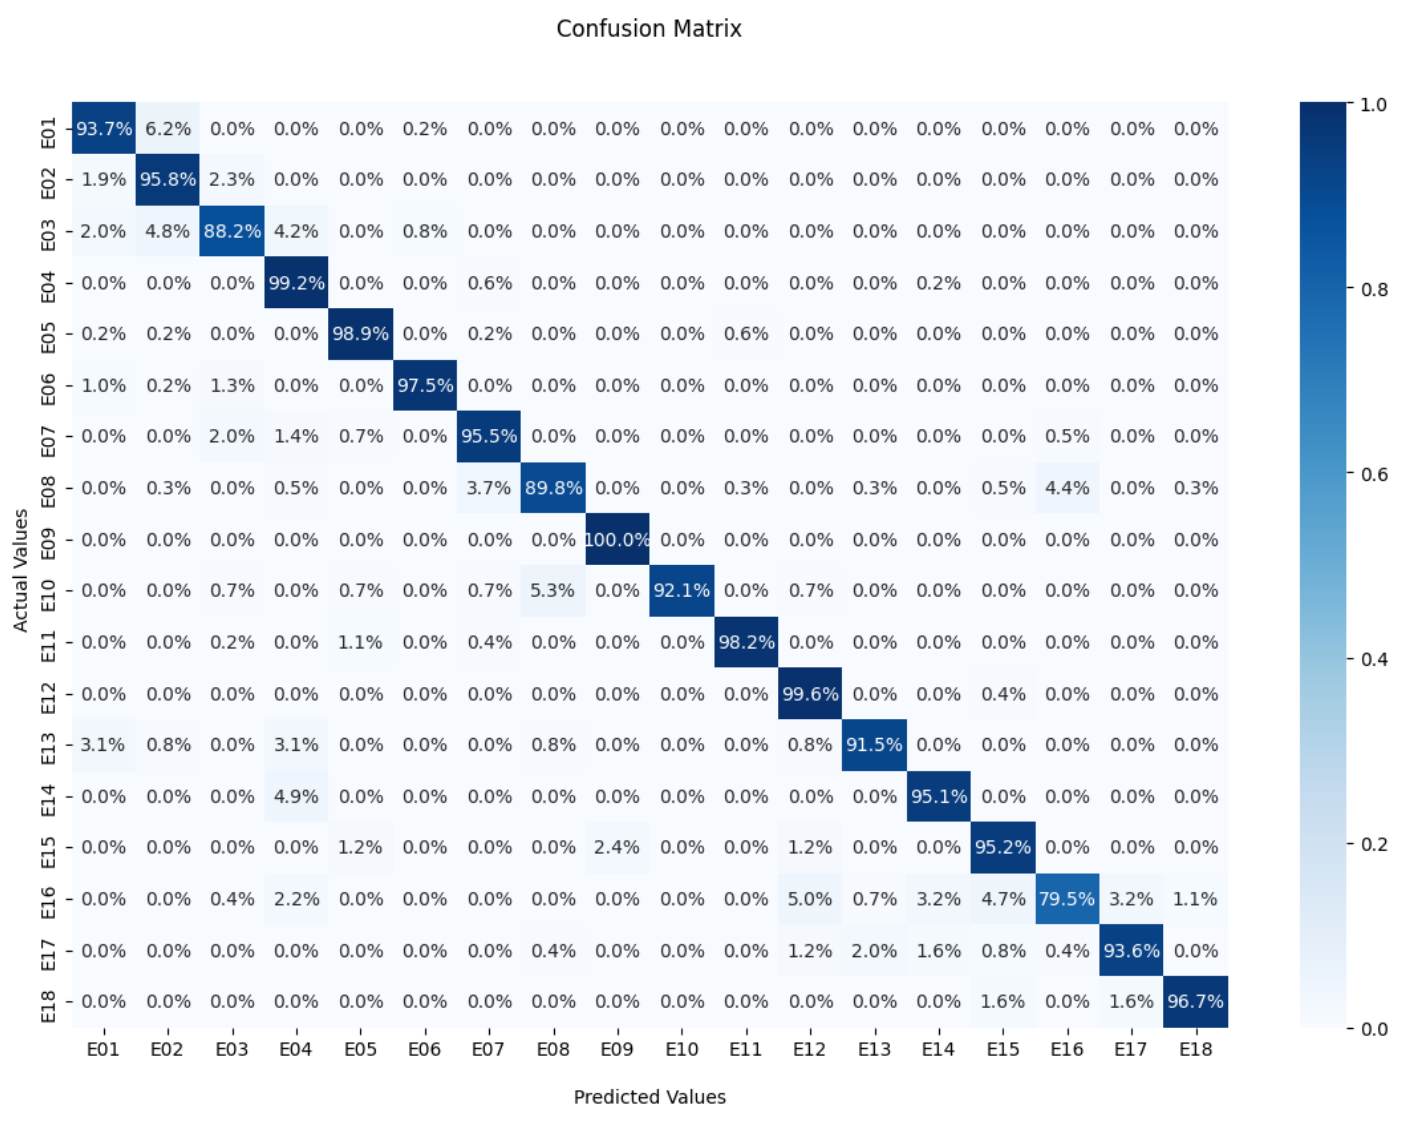
\includegraphics[width=\linewidth]{Figures/validation.png}
    \caption{Confusion Matrix for the Validation Set}
    \label{fig:cfmat-val}
\end{figure}

Furthermore, we additionally verify the accuracy of the data obtained from the test set. The metrics gathered in this stage are presented in Table \ref{tab:metrics-test}. Once again, the system accurately identified the correct classification with an accuracy rate of 90\%. The lowest accuracy achieved by a single class in this situation was 83\%. The global average achieved a minimal drop in the validation set's result, remaining at 93.7\%. These results provide proof that the algorithm demonstrates satisfactory generalization capabilities when making predictions on previously unknown data. The results collected in this stage are displayed in Figure \ref{fig:cfmat-tst} and Table \ref{tab:metrics-test}.

\begin{table}[h!]
\centering
\caption{Classification Metrics for the Test Set}
\label{tab:metrics-test}
\resizebox{.7\linewidth}{!}{%
\begin{tabular}{lllll}
\hline
\textbf{Activity} & \textbf{Precision} & \textbf{Recall} & \textbf{F1-Score} & \textbf{Support} \\ \hline
Stand & 0.91 & 0.90 & 0.91 & 735 \\
Sit & 0.92 & 0.83 & 0.87 & 732 \\
Talk-sit & 0.78 & 0.97 & 0.87 & 747 \\
Talk-stand & 0.97 & 0.96 & 0.96 & 774 \\
Stand-sit & 0.97 & 0.98 & 0.98 & 714 \\
Lay & 0.97 & 0.90 & 0.94 & 678 \\
Lay-stand & 0.96 & 0.99 & 0.97 & 623 \\
Pick & 0.98 & 0.97 & 0.98 & 450 \\
Jump & 1.00 & 1.00 & 1.00 & 211 \\
Push-up & 0.97 & 0.97 & 0.97 & 183 \\
Sit-up & 0.98 & 0.94 & 0.96 & 498 \\
Walk & 0.90 & 0.95 & 0.92 & 307 \\
Walk-backwards & 0.99 & 0.97 & 0.98 & 129 \\
Walk-circle & 0.88 & 0.88 & 0.88 & 127 \\
Run & 0.96 & 0.83 & 0.89 & 269 \\
Stair-up & 0.99 & 0.93 & 0.96 & 348 \\
Stair-down & 0.98 & 0.95 & 0.96 & 307 \\
Table-tennis & 0.95 & 0.98 & 0.97 & 481 \\ \hline
Macro Avg. & 0.95 & 0.94 & 0.94 & 8313 \\
Weighted Avg. & 0.94 & 0.94 & 0.94 & 8313 \\ \hline
Global Average: & \multicolumn{4}{l}{93.7 \%} \\ \hline
\end{tabular}%
}
\end{table}

\begin{figure}[h!]
    \centering
    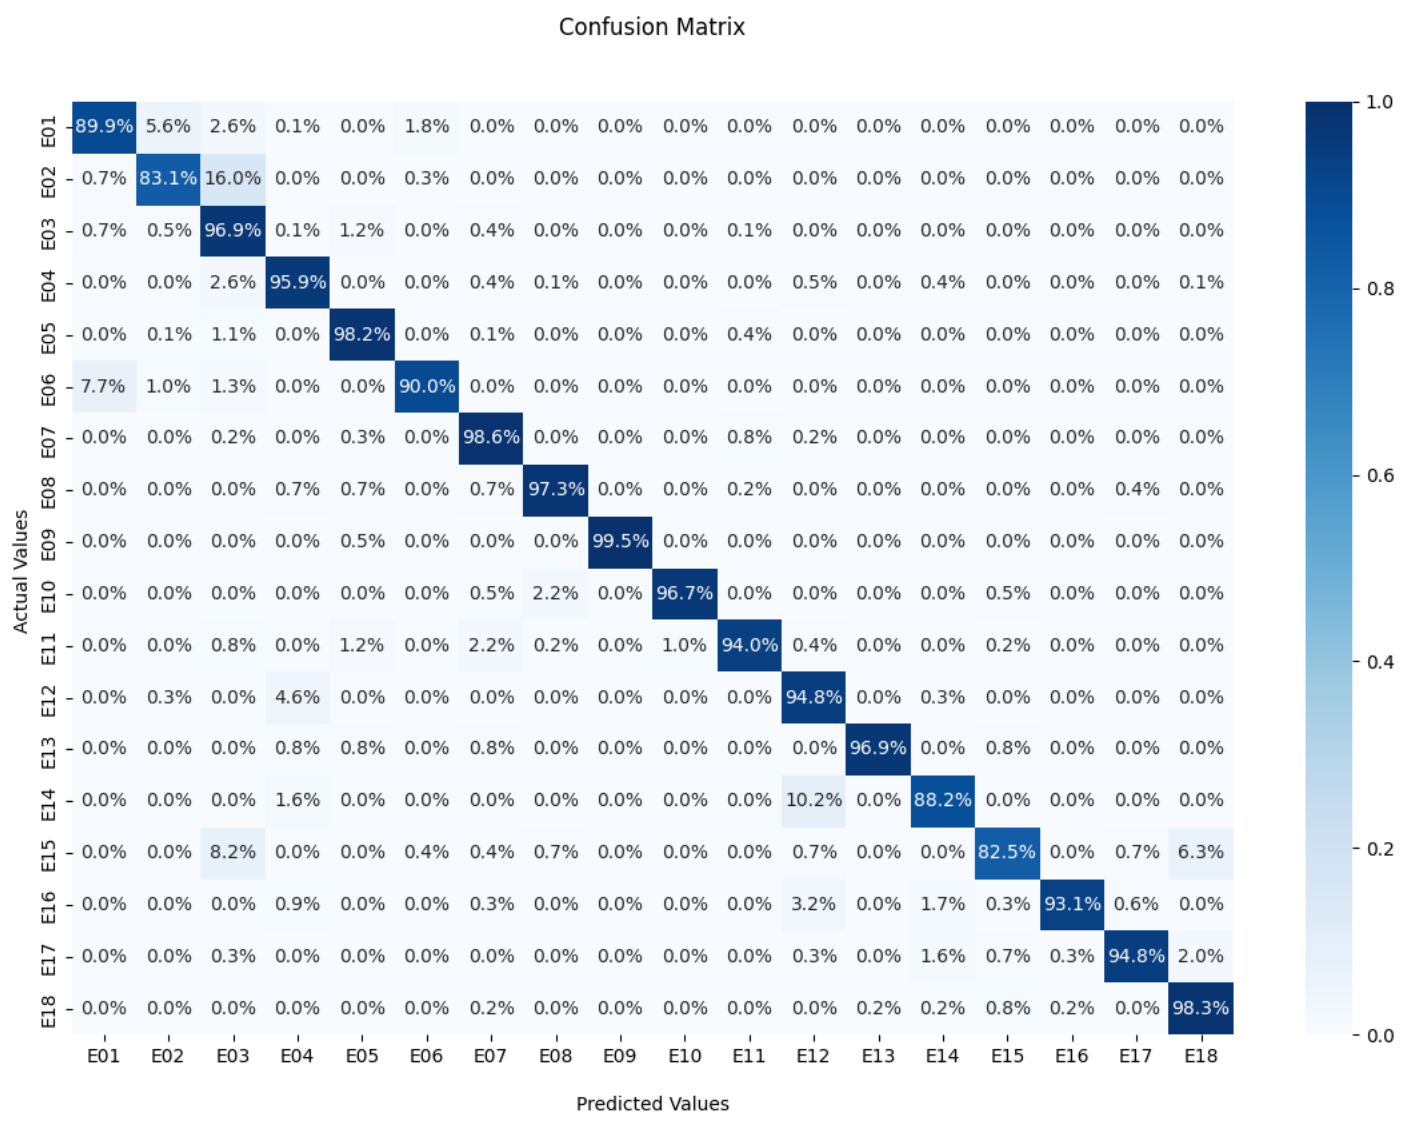
\includegraphics[width=\linewidth]{Figures/test.png}
    \caption{Confusion Matrix for the Test Set}
    \label{fig:cfmat-tst}
\end{figure}

Both tests exhibit a minimum global accuracy of 94\%. These findings validate the viability of this algorithm as a predictive tool for determining the specific activity being performed by users of wearable devices. It is essential to comprehend the system's behavior from both the cloudlet and mobile edge perspectives.

\subsubsection{Architecture Evaluation}

Upon assessing the method, we further examined the number of distinct persons that may be analyzed by each modality of edge computing. We employed both a cloudlet-like architecture and a mobile edge device to evaluate the system. We conducted a test on both devices using the 8313 samples from the test set.

The preliminary experiments were carried out in the cloudlet test environment. We conducted the test and recorded the duration of each forecast. The mean forecast time was 6.7 milliseconds with a standard deviation of 0.2 milliseconds. Based on this outcome, the cloudlet system can handle a maximum of 71 people, as determined by the measure defined in Equation \ref{eq:limit}. The distribution of these periods is depicted in Figure \ref{fig:cloudlet-times}.

\begin{figure}[h!]
    \centering
    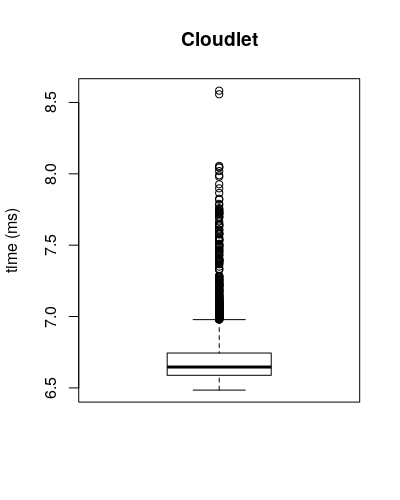
\includegraphics[width=.4\linewidth]{Figures/cloudlet-times.png}
    \caption{Times measured from the Cloudlet}
    \label{fig:cloudlet-times}
\end{figure}

Subsequently, we conducted timing tests on the mobile edge devices. Once again, we conducted the test and recorded the duration for each forecast. The mean forecast time was 42.3 $\pm$ 0.9 ms. Based on this outcome, the maximum number of users that may be accommodated by the cloudlet system using this model is 11. The distribution of these times is depicted in Figure \ref{fig:medge-times}.

\begin{figure}[h!]
    \centering
    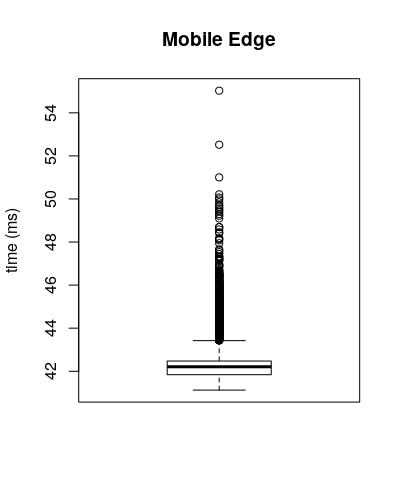
\includegraphics[width=.4\linewidth]{Figures/mobileedge-times.png}
    \caption{Times measured from the Mobile Edge Device}
    \label{fig:medge-times}
\end{figure}

Ultimately, we graphed the data for both tests in parallel to gain a visual understanding of their relationship. Figure \ref{fig:compare-times} illustrates the comparison of various tests. As seen, both the mean and standard deviation are greater in the mobile edge device. This outcome is anticipated, given that the computational capacity of this device is inferior to that of the cloudlet.

\begin{figure}[h!]
    \centering
    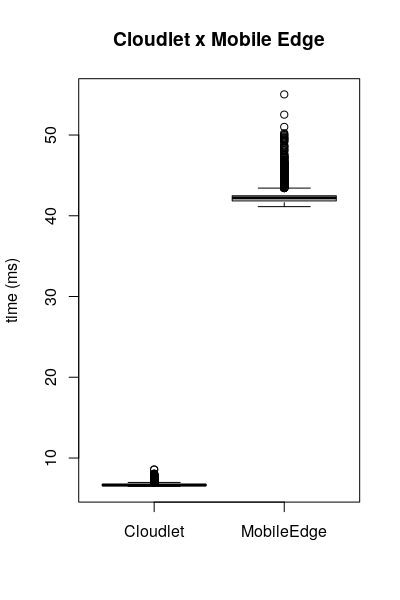
\includegraphics[width=.4\linewidth]{Figures/time-compare.png}
    \caption{Comparison from the measurements in both tests}
    \label{fig:compare-times}
\end{figure}

\subsubsection{Discussion}

During the initial round of tests, our goal was to assess the effectiveness of the proposed method based on its machine-learning metrics. In this regard, we assessed the \textit{Precision}, \textit{Recall}, and \textit{F1-Score} metrics for each class, as well as the overall average precision. 

The experiments demonstrate the viability of this algorithm in executing this task effectively. The method exhibited comparable performance on both the train and validation sets, yielding satisfactory results that are in line with the latest advancements in the field. In addition, we offer a thorough analysis of these indicators, addressing the lack of clarity found in most studies utilizing this dataset.

Subsequently, we assessed the asymptotic threshold for this program to run without any loss of data, taking into account a soft real-time situation. We have established a metric that quantifies the theoretical maximum limit, enhancing the ability to make 97.8\% of forecasts without any loss of data. Unsurprisingly, the cloudlet infrastructure exhibited superior performance in comparison to the mobile edge device. However, employing mobile edge computing remains appropriate for limited populations.

\cleardoublepage
